\chapter{Marco Teórico} \label{chap:marcoteorico}

En este capitulo se desarrollará las bases teóricas y los conocimientos necesarios para poder entender las diferentes terminologías utilizadas en el trabajo de investigación realizado. Se tratará de dar un enfoque simplificado de temas como el sensado remoto,  aprendizaje automático y redes neuronales.

\section{Sensado remoto}\label{sec:sensadoremoto}

En esta sección vamos a realizar una introducción del proceso llevado a cabo para la obtención de una imagen satelital. Comenzaremos desarrollando desde como formamos una imagen satelital, cuales son los rango de bandas, que instrumento se utiliza y los datos en el cual se trabaja.

\subsection{Teledetección}\label{sub:teledeteccion}

La teledetección o \textit{sensado remoto} es el proceso que nos permite obtener una imagen de la superficie terrestre de forma remota, es decir sin estar en contacto con ella. Una imagen satelital es una representación de estos datos reflejados por la superficie terrestre que son captadas por un sensor que se encuentran a bordo de un satélite artificial (fig: \ref{Fig:teledeteccion}). La teledetección no es mas que la detección de propiedades relevantes del entorno, esta capacidad no es despreciable, nos permite desarrollar aplicaciones practicas con un impacto cada ves mayor \citep{percepcion}.

En general la teledetección es la medición de energía emanada de la superficie terrestre. Existen diferentes fuentes de energía, si la fuente de energía es el sol la llamamos \textit{teledetección pasiva}, si la energía medida no es emitida por el Sol es decir es emitida por un sensor la llamamos \textit{teledetección activa} como por ejemplo los sensores de radar que funcionan en el rango de microondas.

Los componentes básicos de un sistema de teledetección incluye lo siguiente \citep{chuvieco}: \textit{fuente de energía},  radiación electromagnética que capta el sensor puede tratarse de una fuente pasiva o activa; \textit{cubierta terrestre}, rasgos naturales o 
realizados por el hombre que refleja el sensor como por ejemplo construcciones; \textit{sistema sensor} compuesto por cámaras, radar, etc  y la plataforma en la que esta puesto (satélite, avión, globo) capta la energía proveniente de la tierra y la almacena o envía al sistema de recepción; \textit{sistema de recepción} encargado de recibir la información proveniente del sensor y almacenar en un formato apropiado para luego ser distribuido a los usuarios; \textit{interprete} es el encargado de manipular los datos de acuerdo a la temática de interés (agricultura, catastro, etc), es decir aplica diferentes niveles de procesamiento sobre los datos crudos obtenidos por el sensor por ultimo tenemos los \textit{usuarios finales} que son los consumidores de la imagen adquirida.

\begin{figure}[H] \centering
  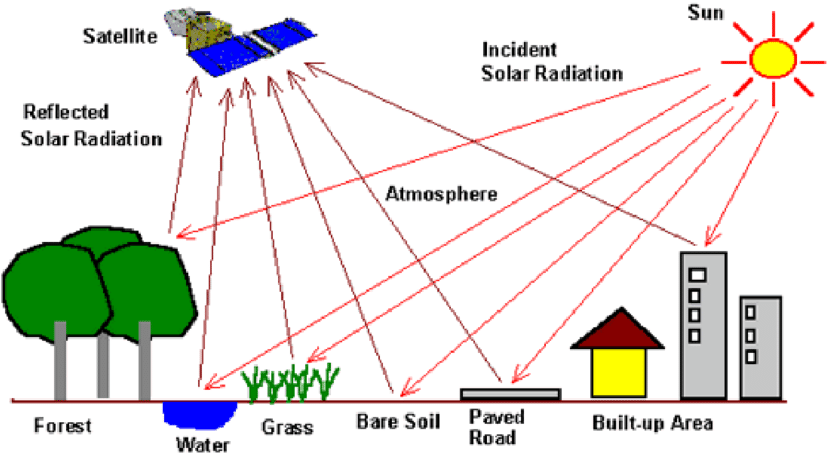
\includegraphics[scale=0.35, keepaspectratio=true,clip=true]{imagenes/MarcoTeorico/teledeteccion.png}
  \caption{Ejemplo de fuente de energía pasiva o activa en teledetección.}\label{Fig:teledeteccion}
\end{figure}

Los tipos de sensores existentes son los  \textit{sensores pasivos}, son aquellos que reciben las señales emitidas naturalmente que fueron reflejadas por los objetos. Sensores como ASTER, MODIS, VIIRS, LandSat son sensores pasivos en la cual la señal se produce por medio de la radiación solar. A su ves existen los \textit{sensores activos} que son aquellos que emiten radiación dirigida hacia un objetivo especifico, esta radiación reflejada del objeto es detectada y medida por el sensor. Ejemplo: Radar, Sonar.

Otras de las características de los sensores son el tipo de imagen que proporciona; estas características vienen definidas por el tipo de resolución; estas resoluciones la podemos definir de la siguiente manera: \textit{resolución espacial}: distancia que corresponde a la unidad mínima de información incluida en un píxel, a menor tamaño de píxel mayor sera la resolución espacial esto quiere decir que el sensor tendrá mayor detalle de los objetos como se puede observar en la figura (a) \ref{Fig:resoluciones};  
\textit{resolución espectral}: la resolución espectral especifica el numero y la anchura de las bandas espectrales que puede ser discriminadas por el sensor (fig: (c) \ref{Fig:resoluciones}); \textit{resolución radiometrica}: indica el numero de bits utilizados para expresar los datos recogidos por el sensor (fig: (b) \ref{Fig:resoluciones}), mayormente cuando es mas grande el número de niveles mayor es el detalle con la cual se podrá expresar dicha información por ejemplo los sensores Landsat (5 y 7) utilizan 8 bits lo que da 2**8= 256 niveles de energía que pueden ser captados; por ultimo tenemos la \textit{resolución temporal}: es el tiempo necesario que tarda el satélite en volver a visitar la misma zona de la Tierra, es decir la periodicidad con la que éste adquiere la misma imagen, este ciclo de cobertura esta en función de el tipo de orbita de la plataforma así como del sensor (alta resolución temporal (< 1 día - 3 días), media resolución temporal (4 - 16 días), baja resolución temporal (> 16 días)).


\begin{figure}[htbp]
\centering
\subfigure[]{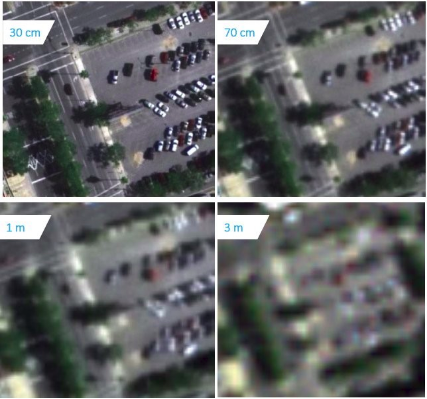
\includegraphics[width=5cm, height=5.1cm]{imagenes/MarcoTeorico/resolucion.png}}
\subfigure[]{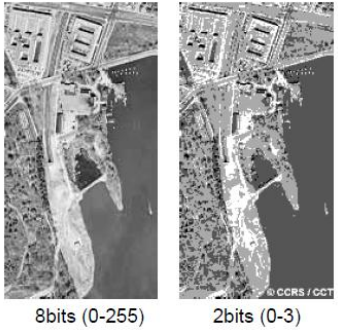
\includegraphics[width=5cm, height=5.1cm]{imagenes/MarcoTeorico/resolucion_radiometrica.png}}
\subfigure[]{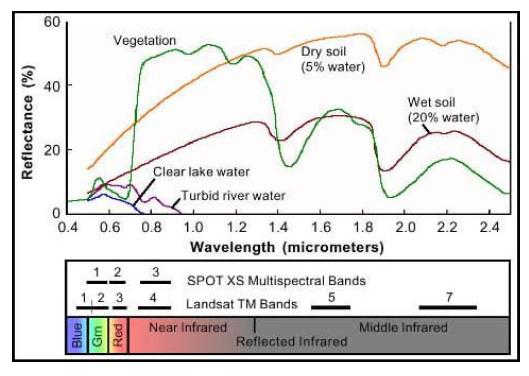
\includegraphics[width=6.6cm,height=5.2cm]{imagenes/MarcoTeorico/resolucion_espectral.jpg}}

\caption{(a) resolución espacial, (b) resolución radiometrica, (c) resolución espectral}\label{Fig:resoluciones}
\end{figure}


\subsubsection{Espectro electromagnético}

En teledetección el espectro electromagnético se denomina al conjunto de todas las longitudes de onda \citep{chuvieco}. Las ondas electromagnéticas cubren una amplia gama de frecuencias o de longitudes de ondas y pueden clasificarse según su principal fuente de producción. 

Las regiones utilizadas para la observación remota de la tierra son: \textit{espectro visible} (0.4 - 0.7 µm): rango de frecuencias del ojo humano, máxima radiación solar, subdividido en tres bandas; rojo (0.6 - 0.7 µm), verde (0.5 - 0.6 µm) y azul (0.4 - 0.5 µm). El \textit{infrarrojo cercano} (0.7 - 1.1 µm) denominado IR fotográfico o reflejado, energía solar que reflejan los cuerpos, su comportamiento es similar al espectro visible. El \textit{infrarrojo medio} (1.1 – 8 µm) se entremezclan radiación solar y emisión, la atmósfera afecta sensiblemente, aprovechado para medir concentraciones de vapor de agua, ozono, aerosoles, etc. El \textit{infrarrojo térmico} (8 - 14 µm) las radiaciones emitidas por los propios cuerpos, se puede determinar la temperatura de un cuerpo (IR térmico), con este tipo se puede disponer de imágenes a cualquier hora del día. Las \textit{microondas} (1mm-1m) son de interés creciente de la teledetección, en esta banda las perturbaciones atmosféricas son menores y es transparente a las nubes, se suelen utilizar en sensores activos. 


\begin{figure}[H] \centering
  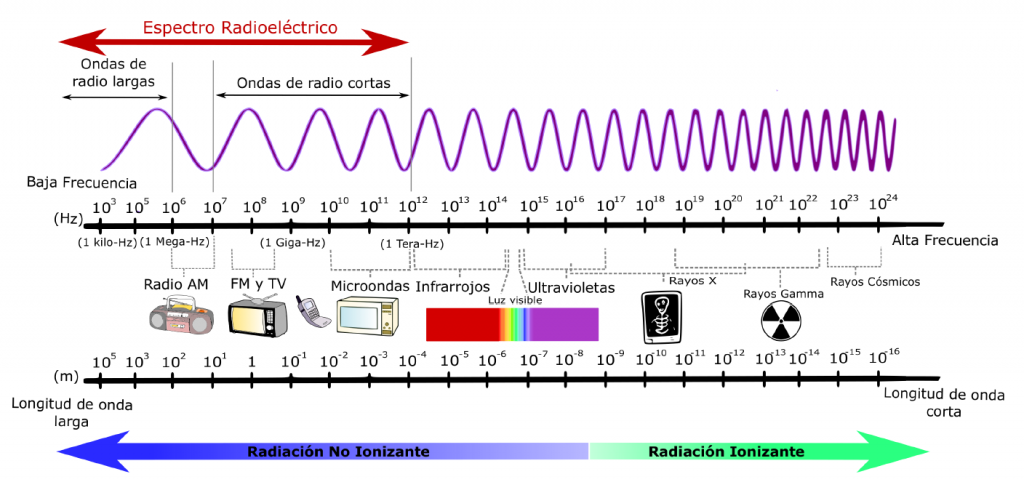
\includegraphics[scale=0.5,keepaspectratio=true,clip=true]{imagenes/MarcoTeorico/espectro-electro.png}
  \caption{Longitudes de onda del espectro electromagnético para diferentes tipos de aplicaciónes.}\label{Fig:espectro-electromagnetico}
  %  https://iie.fing.edu.uy/proyectos/esopo/eem/.}
\end{figure}



\subsection{Adquisición y procesamiento de imágenes satelitales}\label{sub:imagen_satelital}

Las imágenes generadas a partir de la cámara a bordo de un satélite nos brinda información dentro de diversas áreas de estudio, una imagen satelital se compone de diferentes matrices en el cual cada celda representa un píxel, la dimensiones de esta matriz depende del tipo de resolución espacial como se mencionó anteriormente. Los sensores de los satélites almacenan la radiación electromagnética proveniente de distintas coberturas y las guarda en el píxel de acuerdo a los intervalos de onda correspondiente de cada sensor. Esta energía electromagnética se representa en cada píxel por un valor digital llamado Nivel Digital (ND), la cantidad de ND que se podrá representar depende de la resolución radiométrica.

La asignación de colores más conocida por los usuarios es el \textit{falso color} (RGB, por rojo, verde y azul en sus denominaciones en ingles), la cual asigna el color azul a la banda del verde, el color verde a la banda del rojo y el color rojo a la banda del infrarrojo cercano. La información obtenida de diferentes combinaciones de bandas depende del objeto de estudio que se esta llevando a cabo.

%https://acolita.com/wp-content/uploads/2018/01/Teledeteccion_espacial_ArcGeek.pdf
%https://mundosigs.wordpress.com/2016/03/07/que-son-los-sensores-remotos/
%https://www.slideshare.net/noldinn/fundamentos-deteledeteccionemiliochuvieco

Para lograr que la imagen obtenida a partir de una cámara a bordo de un satélite sea información de calidad se debe procesar los datos que deseamos obtener, uno de los requerimientos principales para obtener datos de calidad es que la cámara a bordo este calibrada y sea posible establecer una relación \textit{espacial} y \textit{temporal} de los valores adquiridos por la misma.

Como se desarrollo en el primer capítulo, el objetivo de esta tesis es lograr obtener estas características de manera automática, para esto proponemos el uso de técnicas de \ac{ml} para la resolución de este problema. En la sección siguiente vamos a desarrollar mas en detalle  el concepto \ac{ml} y sus usos.

%http://sedici.unlp.edu.ar/bitstream/handle/10915/20976/Documento_completo.pdf?sequence=1
%http://ing.unne.edu.ar/dep/goeciencias/fotointer/pub/teoria2011/parte02/tdi.pdf



\section{Aprendizaje automático}\label{sec:machinelaerning}

Aprendizaje automático (\ac{ml} por sus siglas en ingles) es una rama de la inteligencia artificial que tiene como objetivo desarrollar técnicas que ayuden a las computadoras aprender determinado comportamiento a partir de los datos de entrada, con el uso de \ac{ml} abordamos tareas que son muy difíciles de resolver con programas escritos y diseñados por seres humanos. Los algoritmos de \ac{ml} juegan un rol importante en diversos campos como \textit{minería de datos}, \textit{reconocimiento de imagen} entre otros dominios, por medio de modelos predictivos nos permite realizar inferencias sobre valores nuevos. 

El principal objetivo de este aprendizaje es desarrollar la capacidad de generalizar y asociar a partir de los datos. Los algoritmos de  \ac{ml} se dividen en dos grandes categorías que son \textit{Aprendizaje supervisado} y \textit{Aprendizaje no supervisado},  en esta tesis desarrollaremos la primer categoría.  El aprendizaje supervisado los datos deben estar previamente etiquetado, es decir que deberá haber una etiqueta por cada característica que deseamos aprender por ejemplo color, tamaño, forma, etc. En un algoritmo de \ac{ml} los datos que usamos para que aprenda y generalice se los llama \textit{datasets de entrenamiento} o \textit{conjunto de entrenamiento}.

Partiendo de los datos de entrenamiento mencionado previamente un algoritmo de \ac{ml} debe aprender una función  $ f(X)$, donde $ X$ representa nuestro conjunto de entrenamiento, la función aprendida por el algoritmo la llamaremos modelo  que retornará un valor $(y)$ tal que se asemeje a la salida que estamos esperando. Para poder llevar a cabo esta tarea el algoritmo debe aprender los parámetros de la función que permita realizar esta aproximación 

El método que nos permite realizar esta aproximación es la \textit{función de costo} (sec.\ref{sub:funcion_costo}), la cual va a  determinar cuan errónea es nuestra salida con respecto a los valores esperado de  $y$, esta etapa la llamamos \textit{entrenamiento de modelo}, su propósito es generar valores lo suficientemente \textit{cercanos} a la respuesta correcta minimizando el error en la predicción medido por la función de costo. Los algoritmo de \ac{ml} son métodos iterativos por lo que en cada iteración debemos minimizar el error obtenido, para poder lograrlo debemos buscar valores óptimos que permitan disminuir el error,estos algoritmos se los conoce como métodos de optimización (sec.\ref{sub:gradient-desc}) y son muy fundamentales en el campo de \ac{ml}. Una vez obtenido un valor de error definido previamente el modelo aprendido debe ser capaz de recibir un nuevo dato que nunca vio el modelo y poder asociar las etiquetas aprendidas de manera automática. 

En esta tesis se abordará los algoritmos de aprendizaje supervisado, en secciones siguientes vamos a desarrollar con mas detalle el proceso de aprendizaje centrándonos principalmente en el problema de clasificación, desarrollando los tipos de clasificadores existentes, la función de costo y el algoritmo de optimización \textit{gradient descent} \citep{cnns}, finalizando con métodos de validación de modelos en \ac{ml}.

\subsection{Aprendizaje supervisado y el problema de la clasificación}\label{sub:aprendizaje_supervisado}
% http://www-bcf.usc.edu/~gareth/ISL/ISLR%20Seventh%20Printing.pdf

Como se desarrollo anteriormente en este trabajo se abordará un problema de clasificación con aprendizaje supervisado. Definimos  el aprendizaje supervisado como una de las tareas mas frecuente en sistemas de \ac{ml}, el aprendizaje supervisado permite a partir de datos conocidos aprender el comportamiento de los mismos, es decir por cada observación de los datos tenemos asociado un valor (etiqueta) que identifica la respuesta correcta que toma nuestros datos, a partir de estos pares de datos el algoritmo debe modelar su comportamiento. 


Entrenar un modelo de clasificación supervisado requiere al menos tres valores:  \textit{datos de entrada}, \textit{salida esperada} y una \textit{función de costo}.  Los datos de entrada son aquellos ejemplos que el algoritmo debe aprender, el objetivo es crear un modelo que generalice para nuevos datos que nunca vio, los datos de entrada deberán ser representativo del mundo real, por ejemplo para una tarea de clasificación entre perros y gatos los datos de entrada deben ser imágenes que pertenezcan a las categorías mencionadas; para resolver un problema de reconocimiento de voz los datos de entrada deben ser audio de personas hablando. Los datos de salida son los valores etiquetados dado un valor de entrada es decir siguiendo el ejemplo anterior para un problema de clasificación entre perros y gatos debemos tener etiquetada cada imagen para saber a que clase pertenece la misma, en reconocimiento de voz cada audio debe tener una transcripción del mismo. El tercer punto es tener una función de costo (\ref{sub:funcion_costo}) que nos permita calcular y evaluar  los resultados de la predicciones obtenidas por los modelo, es decir obtener el error entre la salida esperada y los valores que el modelo predijo.

Siguiendo con lo mencionado en el párrafo anterior los algoritmos de clasificación calculan la probabilidad de cada clase y luego esas probabilidades se mapean y  clasifican las observaciones, a modo de ejemplo en la figura \ref{Fig:clasificacion} se visualiza un modelo de clasificación donde se  genera una frontera que separa los datos rojos y verdes, la linea punteada en este caso sera la función que el modelo deberá aprender. El proceso de entrenamiento implica los siguiente pasos, dado un conjunto de imágenes de entradas $X$ y uno de salidas esperadas $Y$ (etiquetas de la clase) se cuenta con un conjunto de $N$ pares anotados ${(x_i, y_i)}_{i=1,..,N}$  que a través de un algoritmo de aprendizaje debemos encontrar una relación de una función que se aproxime a los datos etiquetados de la siguiente forma: $f(X) ≈ Y$. La función $f(X)$ es un modelo paramétrico que a partir de un conjunto finitos de parámetros permite realizar la predicción de un valor dado, es decir dado un modelo paramétrico como por ejemplo uno lineal de la forma $y_i = w^t x_i + \epsilon_i$ en donde $\epsilon_i$ es el error del modelo e $Y$ puede tomar valores $(-1,1)$ para un problema de clasificación binaria, lo que se busca es por medio de un modelo de aprendizaje encontrar los valores de  $w$ que se aproxime a los valores $y_i$.

En el estado del arte existen diversos algoritmos para resolver el problema de clasificación utilizando \ac{ml}, en la siguiente sección se desarrollará en mas detalle, en esta tesis nos enfocaremos en los clasificadores llamados maquina de vectores de soporte. 

\begin{figure}[H] \centering
  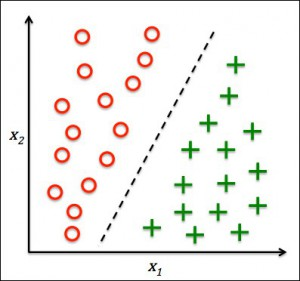
\includegraphics[scale=0.4,keepaspectratio=true,clip=true]{imagenes/MarcoTeorico/classification.jpg}
  \caption{La linea punteada es una función que indica la separación entre dos clases.}\label{Fig:clasificacion}
\end{figure}




\subsection{Modelos de clasificación}\label{sub:clasificadores}

En base a lo desarrollado en la sección anterior (sec.\ref{sub:aprendizaje_supervisado}) podemos definir diferentes algoritmos de clasificación que se utilizan en la actualidad.

%LOG_reg https://medium.com/datos-y-ciencia/aprendizaje-supervisado-introducci%C3%B3n-a-la-clasificaci%C3%B3n-y-principales-algoritmos-dadee99c9407
\par \textbf{Regresión Logística}: describe y estima la relación entre una variable binaria dependiente y variables independiente. El objetivo de este método es encontrar un modelo que describa la relación entre la respuesta del modelo con las variables independientes (variables predictivas o explicativas). En un modelo de clasificación por regresión logística el valor $z$ de la ecuación \ref {ecu:rg} es una combinación lineal de los pesos y las característica $x_i$, definido como $z=w^t x_i$. 
   

\begin{equation}\label{ecu:rg}
\phi(z) = \frac{1}{1+e^{-z}}.
\end{equation}

La salida de la función sigmoide $\phi(z)$ (\ref {ecu:rg}) se interpreta como la probabilidad de que un valor determinado pertenezca a una de las clases, es decir:
\begin{equation}\label{ecu:f_sig_class}
\hat{y} = \left \{\begin{matrix} 1 & \mbox{si }\phi(z) \ge 0
\\ 0 & \mbox{si }\phi(z) < 0 \end{matrix}\right. 
\end{equation}


\begin{figure}[H]
 \centering
  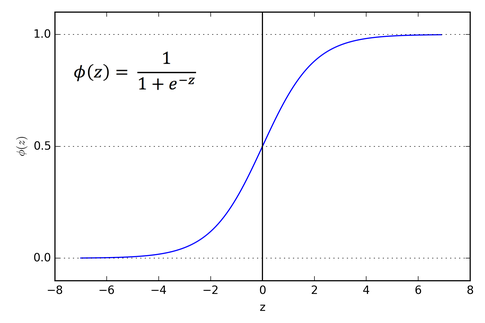
\includegraphics[scale=0.5]{imagenes/MarcoTeorico/sigmoide.png}
  \caption{Regresión Logística, \citep{bishop}.}
  \label{Fig: log_reg}
\end{figure}


\par \textbf{Árboles de decisión}: Estos tipos de clasificadores se forman a partir de  un conjunto finito de valores  que toman la forma/estructura de un árbol desglosando el conjunto de datos de entrada en subconjuntos mas pequeños. El resultado final es un árbol con nodos de decisión y nodos de hoja en donde un nodo de decisión tiene dos o más ramas y un nodo hoja representa una clasificación o decisión. 

Para dar mas detalle en la figura \ref{Fig: decision-tree} tenemos 4 variables de decisión $ X, Y, W, Z$, dado un valor  de entrada en este caso numérico se tomara una decisión en este caso creando dos grupos  si $ X$  es menor a 10 o si es mayor o igual a 10 segmentando el conjunto de datos en dos, de la misma manera las decisiones se tomaran en los nodos $ Y, W, Z$, hasta llegar a la hoja que sera la decisión que debemos tomar. Los árboles de decisión pueden manejar tanto datos categóricos como numéricos.

  
\begin{figure}[H]
 \centering
  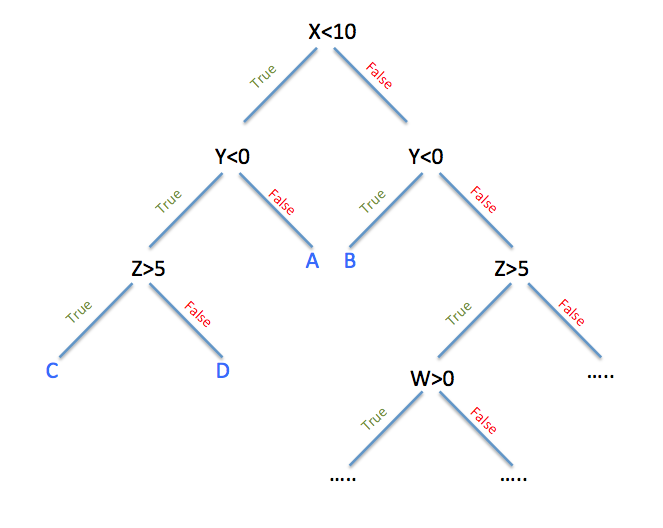
\includegraphics[scale=0.3,keepaspectratio=true,clip=true]{imagenes/MarcoTeorico/decision-tree.png}
  \caption{Arboles de decisión para 4 variables X, Y, W, Z .}% \\ (Adaptado de: https://medium.com/machine-learning-bites)}
  \label{Fig: decision-tree}
\end{figure}


\par \textbf{Bosques Aleatorios, (RF por su denominación en ingles)}: Este  algoritmo combina diferentes algoritmos de igual o diferentes tipos para realizar la clasificación, son llamados algoritmos de ensamble. Por ejemplo, ejecutar la predicción sobre un algoritmo de \textit{maquina de vectores de soporte} o  \textit{árboles de decisión} y luego tomar el voto para la consideración final de la clase del objeto que se esta evaluando.  

En la figura \ref{Fig: random_forest} se da un ejemplo de un algoritmo \textit{RF} donde se crea tres \textit{arboles de decisiones} independientes  inicializado aleatoriamente para cada uno de esto tendrá su correspondiente decisión como se describió en el ítem anterior, la proporción de árboles que toman una misma respuesta se interpreta como la probabilidad de la misma.

\begin{figure}[H]
 \centering
  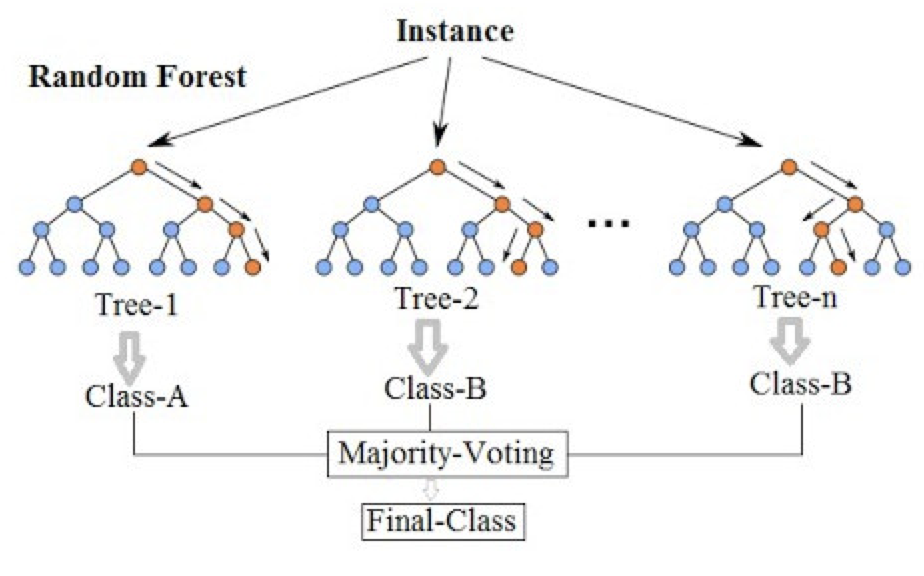
\includegraphics[scale=0.6,keepaspectratio=true,clip=true]{imagenes/MarcoTeorico/random-forest.png}
  \caption{Ejemplo de bosques aleatorios para diferentes clasificadores donde la salida final esta dada en la a proporción de árboles que toman una misma respuesta.} 
  %\\ https://www.researchgate.net/publication/324517994}
  \label{Fig: random_forest}
\end{figure}

\par \textbf{Maquina de vectores de soporte (SVM por su siglas en ingles)}: son otro tipo de clasificadores lineales,  el objetivo de un algoritmo \ac{svm} es construir un hiperplano (\ref{Fig: svm_margen_hiperplano} (a)) en un espacio de $n$ dimensiones que permita separar de manera optima dos datos de una clase con respecto a la otra. La característica fundamental de \ac{svm} es encontrar el hiperplano que tenga la máxima distancia, \textit{margen} , entre los puntos que estén más cerca de el mismo. El margen se define como la distancia perpendicular entre el límite de decisión y el punto de datos más cercano, como se muestra en la figura \ref{Fig: svm_margen_hiperplano} (b)}. La ubicación de este límite está determinada por un subconjunto de los puntos de datos, conocidos como vectores de soporte \citep{bishop}.


% http://bibing.us.es/proyectos/abreproy/70448/fichero/05_Capitulo4.pdf
%http://zaguan.unizar.es/record/59156/files/TAZ-TFG-2016-2057.pdf?version=1

%https://www.cienciadedatos.net/documentos/34_maquinas_de_vector_soporte_support_vector_machines
%pag.326 y 328 nuevo de bishop


\begin{figure}[htbp]
\centering
\subfigure[]{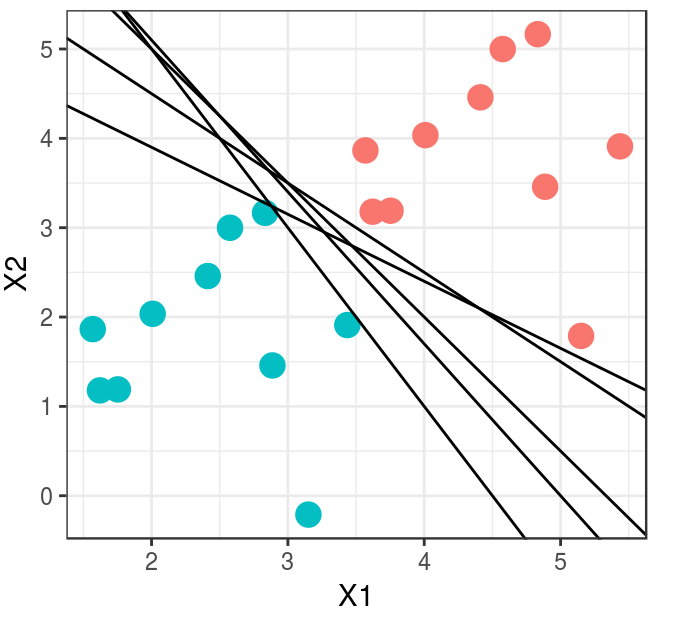
\includegraphics[width=6cm, height=6cm]{imagenes/MarcoTeorico/hiperplanos.png}}
\subfigure[]{\includegraphics[width=5.5cm, height=6cm]{imagenes/MarcoTeorico/margen_svm.png}}

\caption{(a) Hiperplanos de seaparación (b) margen de separacion del hiperplano.}\label{Fig: svm_margen_hiperplano}
\end{figure}

Para un problema de clasificación binaria en el que necesitamos separar dos clases, existen muchos hiperplanos posibles \ref{Fig: svm_margen_hiperplano} (a), como se desarrollo anteriormente el objetivo es encontrar un plano que logre el margen máximo entre dos puntos de datos de ambas clases; vamos a dar considerar un modelo de clasificación lineal con etiquetas $t_n \in\{1, -1 \}$ y datos de entrenamiento de $N$ vectores de entada $x_i,..., x_n$ \eqref{eq: modelo-lineal}.

\begin{equation}\label{eq: modelo-lineal}
    y(x) = w^{\rm T} f(x) + b.
\end{equation}

Dado este conjunto de datos asumimos que son lineal mente separables por lo que al menos existe un conjunto de parámetros $w$ y $b$ de modo, $y(x_n) > 0 $ para puntos $t_n = 1 $ y $y(x_n) < 0$ para datos con etiqueta $t_n = -1$. En diversos casos existen $ n$ hiperplanos de separación (a)  \ref{Fig: svm_margen_hiperplano} que permita lograr una solución al problema.  El algoritmo de \ac{svm} trata de resolver este problema calculando el margen de separación entre los datos. Para obtener el hiperplano con mayor margen óptimo se  debe calcular la distancias de cada observaciones a un determinado hiperplano. La menor de estas distancias, conocidas como margen, determina cuan alejado esta el hiperplano de las observaciones, la distancia de un punto al hiperplano viene dada por la siguiente expresión (ec.\eqref{eq: distancia-margen}):

\begin{equation}\label{eq: distancia-margen}
   \frac{t_n y(x)}{ \|w \|}  = \frac{t_n(w^{\rm T} f(x_n) + b)}{ \|w \|}.
\end{equation}

El margen viene dado por la distancia perpendicular al punto más cercano  $x_n$ del conjunto de entrenamiento, y deseamos optimizar los parámetros $ w$ y $ b$ para maximizar esta distancia, así, la solución del margen máximo esta dada por:

\begin{equation}\label{eq: margen-maximo}
\argmax_{w, b} \left\{ \frac{1}{\|w \|} \min_{n} [t_n(w^{\rm T} f(x_n) + b)]  \right\}
\end{equation}

Como podemos ver encontrar un hiperplano optimo es un problema de optimización, la solución directa de este problema de optimización sería muy compleja, entonces podemos convertirlo a un problema equivalente que sea mucho más fácil de resolver reescalando $w \to kw$ y $b \to kb$ entonces la distancia desde cualquier punto $X_n$ hasta la frontera de decisión esta dada por $ t_n y(x_n) / \|w \|$ no cambia, podemos usar esto para establecer en el punto más cercano:

\begin{equation}\label{eq: margen-maximo_2}
t_n(w^{\rm T} f(x) + b) = 1.
\end{equation}
Para todos los puntos de datos tendrán las siguiente restricción:

\begin{equation}\label{eq: margen-maximo_3}
t_n(w^{\rm T} f(x) + b) \geq 1.
\end{equation}

Para este problema de optimización se requiere maximizar $\|w \|^{-1}$, que es equivalente a minimizar $\|w \|^{2}$, por lo que nos queda la siguiente ecuación:

\begin{equation}\label{eq: margen-maximo_optimizacion}
\argmin_{w, b}  \frac{1}{2}} \|w \|^{2}.
\end{equation}

La resolución del problema utilizamos los multiplicadores de Lagrange  \citep{bishop} con valores de $a_n \geq 0$, la función Lagrangiana tendrá la siguiente forma:

\begin{equation}\label{eq: lagrange}
L(w, b, a) = \frac{1}{2}} \|w \|^{2} - \sum_{n=1}^{N} a_n \left\{ t_n(w^{\rm T} f(x) + b)- 1 \right\}.
\end{equation}


En la gran mayoría de casos, los datos no se pueden separar linealmente de forma perfecta, por lo que no existe un hiperplano de separación y no puede obtenerse un margen máximo de manera simple. Una de las estrategias usadas al momento de trabajar con conjuntos de datos no lineales es expandir las dimensiones del espacio, esto se logra transformando o modificando alguna de sus dimensiones. La manera de realizar esta tarea a por medio de la función  \textit{kernel}, esta función permite proyectar un espacio $ X$ a un espacio de mayor dimensionalidad. Existen diversos tipos de \textit{kernel} en la literatura como son los \textit{kernel lineal}, \textit{kernel polinómico}, \textit{kernel gaussiano RBF}, entre otros \citep{SVM}. 


Las ventajas de estos clasificadores son: eficaz para grandes espacios dimensionales, efectivo en casos en los que el número de dimensiones es mayor que el número de muestras, se pueden especificar diferentes funciones del kernel para la función de decisión, el proceso de entrenamiento es más rápido en comparación con otros tipo de clasificadores, sobre todo para cuando tenemos un conjunto de entrenamientos grandes.
%http://scielo.sld.cu/scielo.php?script=sci_arttext&pid=S1684-18592016000300008

\subsection{Función de costo}\label{sub:funcion_costo}
% ENLACES DE INTERES
%http://bibing.us.es/proyectos/abreproy/11185/fichero/Volumen+1_Detector+Multiusuario+para+DS-CDMA+basado+en+SVM%252F7.+Support+Vector+Machines%252FSupport+Vector+Machines.pdf
%https://rpubs.com/Joaquin_AR/267926
%https://medium.com/datos-y-ciencia/aprendizaje-supervisado-introducci%C3%B3n-a-la-clasificaci%C3%B3n-y-principales-algoritmos-dadee99c9407

% FIN

%COST F EN CLASIFICACION.
% https://machinelearningknowledge.ai/cost-functions-in-machine-learning/#Cost_functions_for_Classification_problems
El proceso de aprendizaje de un algoritmo de \ac{ml} genera un  modelo que predice un valor dado a partir de un nuevo dato que nunca vio, para poder realizar esta tarea necesitamos que el algoritmo aprenda los parámetros del modelo para poder aproximar la salida deseada a los valores predichos. La forma de determinar cuan distante y/o diferente es la salida con respecto a los valores esperado es por medio de la \textit{función de costo}, este método permite evaluar qué tan bien el algoritmo modela el conjunto de datos si las predicciones son incorrectas con respecto a los valores deseados. 

Como se desarrollo anteriormente un algoritmo de \ac{ml} deberá minimizar la función de costo para que esta produzca un valor menor de error entre el valor esperado y la salida del modelo. Dependiendo del modelo de clasificación que estemos utilizando existen diferentes funciones de costo que nos permiten calcular el error del modelo; entre ellas están Quadratic cost \citep{quadratic_cost}, Cross-entropy cost \citep{cross_entropy}, Exponential cost \citep{exponential_cost}, Hellinger distance \citep{Hellinger}, Kullback–Leibler divergence \citep{kullback}, entre otras.

%https://stats.stackexchange.com/questions/154879/a-list-of-cost-functions-used-in-neural-networks-alongside-applications

\subsubsection{Optimización de la función de costo} 
%https://hackernoon.com/gradient-descent-aynk-7cbe95a778da
%https://stxlearning.com/2018/03/25/optimizacion-deep-learning-y-complejidad-computacional/
En modelos de \ac{ml} debemos encontrar aquellos parámetros que minimizan la función de costo como se menciono previamente, este es un problema de optimización ya que si encontramos la solución podemos encontrar esos parámetros que disminuyen el error.

La mayoría de los algoritmos de \ac{ml} deben aprender mas de un parámetro, en algunos casos hasta decenas de millones de parámetros, es por esto que todos los algoritmos  son métodos de optimización ya que se busca aprender los parámetros de manera eficiente. La estrategia mas típica para problemas de optimización son los llamados métodos de descenso; dentro de estos se encuentran: descenso de gradiente, descenso de gradiente estocástico y método de Newton Rawson de 2 orden.

\subsubsection{Descenso de gradiente}\label{sub:gradient-desc}
Descenso de gradiente, \textit{gradient descent} en ingles, es un algoritmo de optimización que busca encontrar el mínimo local o global de una función convexa.  En \ac{ml} usamos descenso de gradiente para encontrar los parámetros de nuestro modelo que mejor definen nuestro conjunto de entrenamiento. Este algoritmo es un método iterativo que utiliza el gradiente para definir la dirección que el modelo debe seguir para reducir el error, en cada iteración gradualmente converge hacia un mínimo optimizando los parámetros que minimizan la función de costo. 


\begin{equation}
w^* =  \arg\min_{w} \mathcal{L}(X; w).
\end{equation}

Esto quiere decir que queremos encontrar los parámetros $w$ que minimicen la diferencia entre las salidas $Y$ y las producidas por el modelo dependiente de $w$. Entre menor  diferencia mejor aproximación a la salida $Y$. 

\begin{figure}[H] \centering
  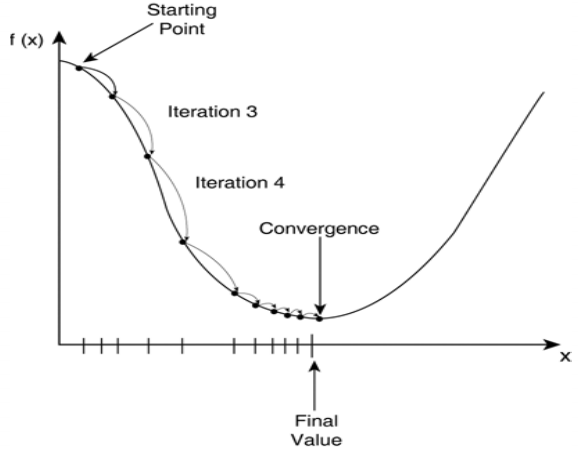
\includegraphics[scale=0.4,keepaspectratio=true,clip=true]{imagenes/MarcoTeorico/gradient-descent.png}
  \caption{Descenso de Gradiente para N iteraciones.}\label{Fig:gradient-descent}
\end{figure}


%Gradiente extraido de :https://www.cs.huji.ac.il/~shais/UnderstandingMachineLearning/understanding-machine-learning-theory-algorithms.pdf
El gradiente de una función diferenciable $ \mathcal{L}: R^d \longrightarrow R $ en $\textbf{w}$, denotado $ \nabla \mathcal{L}(w) $ vector de derivadas parciales de $\mathcal{L}$ es:
\begin{equation}
\nabla \mathcal{L}(x) = (\frac{\partial \mathcal{L}(\textbf{w})}{\partial w_1},....., \frac{\partial \mathcal{L}(\textbf{w})}{\partial w_n}).
\end{equation}

El algoritmo de descenso de gradiente es un método iterativo del cual comenzamos con un valor inicial de $\textbf{w}$, luego en cada iteración damos un paso en la dirección negativa del gradiente en el punto actual, es decir, el paso de actualización es:
\begin{equation}
\textbf{w}^{(t-1)} = \textbf{w}^{(t)} - \alpha \nabla \mathcal{L}(\textbf{w}^{(t)}).
\end{equation}

Donde $ \alpha > 0$, dado que el gradiente apunta en  dirección a la mayor aumento de $\mathcal{L}$ alrededor de $w^{(t)}$, el algoritmo da pequeños paso en la dirección opuesta, disminuyendo así el valor de la función $\mathcal{L}$. El resultado final podría ser el ultimo valor obtenido $w^{(t)}$ o o el valor que genero mejor rendimiento $\arg\min_{t}\mathcal{L}(\textbf{w}^{(t)})$ \citep{gradient_des}.

% PONEMOS BACKPROPAGATION, LEARNING RATE
%http://ruder.io/optimizing-gradient-descent/
%https://turing.iimas.unam.mx/~ivanvladimir/posts/gradient_descent/

En un modelo de aprendizaje automático lo que se busca es encontrar una relación entre los datos de entradas y las salidas deseadas como se menciona anteriormente, por ejemplo para un modelo de la forma $y= mx+b$ (regresión lineal) depende de los parámetros  $m$ y $b$;  estos dos valores los representamos usando la notación $\theta$, de tal forma que buscamos encontrar $\mathcal{L}_{\theta} (X) \approx Y$. Es decir que la función $\mathcal{L}$ con los parámetros $\theta$ de tal forma que para todos los valores $X$ de entrada aproxime a los valores de salida $Y$ correspondientes. 

Para validar que tan bien nuestros parámetros definen a nuestra salida podemos definir una función de costo $J(\theta)$ que mida la diferencia entre las salidas esperadas y las salidas producidas por el modelo. El valor $\hat\theta$ es una nueva posición para los parámetros que se acercan más al mínimo, es decir que hacen que $\mathcal{L}_\theta(X)$ aproxime mejor a $Y$. El algoritmo para el computo del descenso de gradiente tiene la siguiente forma:

%\begin{algorithm}[H] %\caption{Descenso de Gradiente}\label{euclid}
%\begin{algorithmic}[1]

%\State $\textbf{INPUT} \gets (X, Y, \theta,iteraciones, \alpha)$
%\State $\textbf{OUTPUT} \gets \theta $
%\State \textbf{i} = 0
%\While {\textbf{i} <  iteraciones}{
%\State i++
%\State	error = \textit{Función\_Costo}(X, Y, \theta)

%\If {error < min\_error}
%	\State	break
%\Else
%	\State \texttt{\theta_{j} := \theta_{j} - \alpha \frac{\partial}{\partial \theta} J(\theta_{1}, \theta_{0})}
	
%\EndIf
%\EndWhile
%\end{algorithmic}
%\end{algorithm}

\begin{algorithm}[H] \caption{Descenso de Gradiente}\label{euclid}
\begin{algorithmic}[1]
\State \textbf{INPUT} $\gets$ ($\mathcal{L}$, $\theta$, threshold or iters, $\alpha$)
\While {True}
\If {$\theta_{1} - \theta_{0}$  $>$ threshold or iters }
	\State	break
\Else
	\State \texttt{$\hat\theta$ := $\hat\theta$ - \alpha \frac{\partial}{\partial \theta} J(\theta_{1}, \theta_{0})}
	
\EndIf
\State iters += 1
\EndWhile
\end{algorithmic}
\end{algorithm}


Existen diversas variantes de descenso por gradiente como \textit{Batch gradient descent}, \textit{Stochastic gradient descent} y \textit{Mini-batch gradient descent} \citep{variants_gd}.

\subsection{El problema de sobreajuste}\label{sub:validacion-modelo}

En algoritmos de \ac{ml} debemos hacer que nuestro modelo generalice para nuevos valores de entrada desconocidos es por esto que debemos evaluarlo para determinar su comportamiento en base a nuevos datos. Uno de los principales motivos por el cual tenemos que validar nuestro modelo es para obtener una medida de cuan erróneo pueden llegar a ser nuestros resultados en la predicción, esta causa esta dada por dos términos muy importante que debemos tener en cuenta es el \textit{sobreajuste} (overfitting en ingles) y \textit{subajuste} (underfitting en ingles). El valor de overfitting y underfitting son dos grandes problemas en \ac{ml} que influye en la predicción dado un nuevo valor de entrada y es el que debemos atacar. 

El overfitting ocurre cuando un modelo aprende en detalle junto al ruido en los datos de entrenamiento afectando negativamente el rendimiento del modelo en los nuevos datos a predecir, esto significa que el ruido o las fluctuaciones aleatorias en los datos de entrenamiento son aprendidos como conceptos por el modelo. El problema es que estos conceptos no se aplican a los nuevos datos e impactan negativamente en la capacidad de generalización de los modelos.

Como parte opuesta al overfitting esta el  underfitting, este concepto hace referencia a aquellos modelos que no pueden generalizar nuevos datos de entrenamiento de manera correcta. Mayormente en problemas de underfitting se necesita mayores características de los datos para la construcción de los modelos. En la figura \ref{Fig: overUnder} podemos apreciar los enfoques mencionados anteriormente.

\begin{figure}[h]
 \centering
  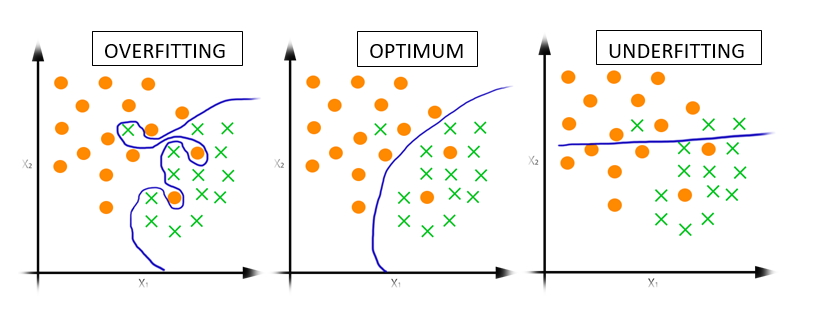
\includegraphics[scale=0.4,keepaspectratio=true,clip=true]{imagenes/MarcoTeorico/OverFUnderF.png}
  \caption{Ejemplo de overfitting (izquierda), modelo óptimo (centro) y underfitting (derecha) }%\\(Adaptado de: https://medium.com/deep-learning-neuroevolution-extreme-learning-machines)}
	\label{Fig: overUnder}
\end{figure}



\subsubsection{Estrategias de aprendizaje para evitar el sobreajuste}

Existen diferentes técnicas para evitar los problemas mencionados en la sección anterior, una de ellas es por  \textit{validación cruzada} (cross validation en ingles). La validación cruzada es una técnica que evalúa los resultados de un análisis estadístico y garantiza de que sean independientes de la partición de los datos de entrenamiento y prueba. 

Hay diversos tipos de validación cruzada de las cuales podemos nombrar:


\par \textbf{Validación cruzada de K vueltas}: consiste en dividir el conjunto de datos en \textit{k} subconjuntos. Existe un $k-1 $ valor que es el de validación, es decir, se toma uno de los subconjunto y se los utiliza como validación y el resto como entrenamiento.  Este proceso se repite durante $k $ iteraciones con cada uno de los subconjunto de dato de validación. Para finalizar se utilizar aquel subconjunto de datos que posea mayor generalidad.
\begin{figure}[H]
 \centering
  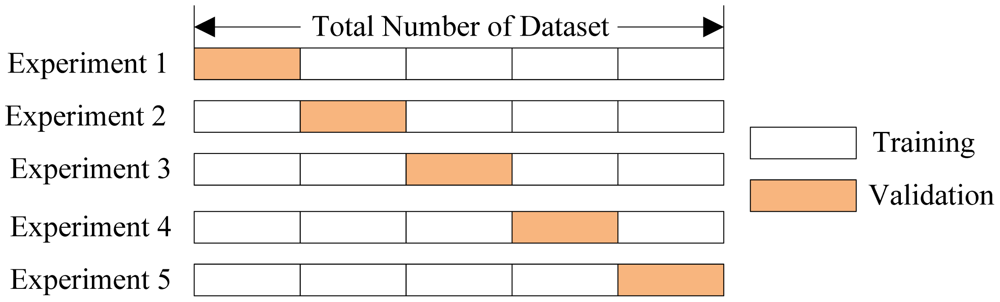
\includegraphics[scale=0.4,keepaspectratio=true,clip=true]{imagenes/MarcoTeorico/crossvalidat.png}
  \caption{Validación cruzada para k=5.}%\\(Adaptado de:{http: //goo.gl/Dp85h3})}
	\label{Fig: crossvalidation}
\end{figure}

\par \textbf{Leave-One-Out Cross-Validation (LOOCV)}: Es un caso particular de validación cruzada, tomamos todos los datos que poseemos y utilizamos solo uno del subconjunto para validar. La ventaja de este método es que usamos todo los datos para realizar el entrenamiento.

\begin{figure}[H]
 \centering
  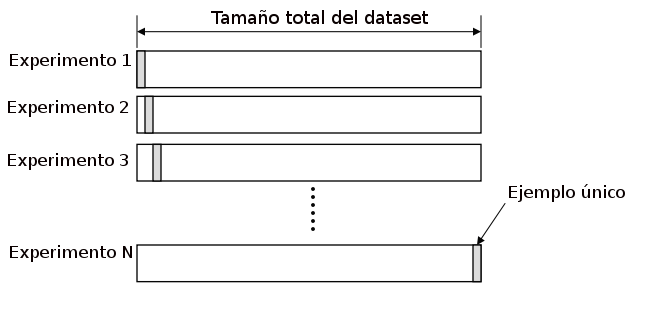
\includegraphics[scale=0.4,keepaspectratio=true,clip=true]{imagenes/MarcoTeorico/cross-validation-LOOCV.png}
  \caption{Leave-One-Out Cross-Validation (LOOCV).}%\\ (Adaptado de: https://sebastianraschka.com/)}
	\label{Fig: crossvalidation-LOOCV}
\end{figure}

\par \textbf{Random Subsampling}: En esta técnica, se eligen aleatoriamente múltiples conjuntos de validación y se combinan para formar un conjunto de datos de prueba. Los datos restantes forman el conjunto de datos de entrenamiento.

\begin{figure}[H]
 \centering
  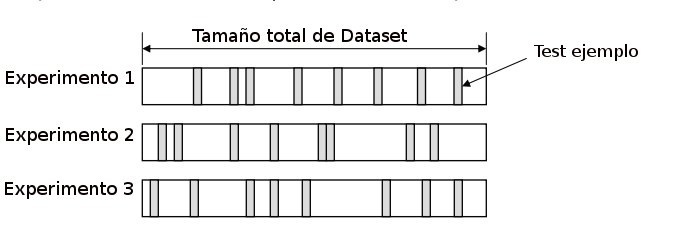
\includegraphics[scale=0.5,keepaspectratio=true,clip=true]{imagenes/MarcoTeorico/cross-validation-random.png}
  \caption{Random Subsampling.}% (Adaptado de: https://sebastianraschka.com/)}
	\label{Fig: random-Subsampling}
\end{figure}

%IMPORTANTE: https://sebastianraschka.com/pdf/manuscripts/model-eval.pdf
%https://dzone.com/articles/machine-learning-validation-techniques

\subsection{Evaluación de modelos}\label{sub:evaluación-modelo}

Cuando entrenamos modelos en \ac{ml} debemos medir la efectividad del mismo, es decir, cual es la capacidad de generalizar dado un conjunto de valores desconocidos. Para poder determinar esta efectividad existen métodos de evaluación que nos permiten obtener el grado de error que hay en el modelo creado.

La forma de validar modelos en \ac{ml} es a través de métricas, la elección de la métrica depende de cada tarea a realizar, es importante revisar este conjunto de métricas para tener la certeza de que nuestro modelo tiene un buen rendimiento. Las métricas de evaluación que utilizamos en esta tesis serán las siguientes \textit{Matriz de confusión}, \textit{accuracy}, \textit{precision}, \textit{recall} y \textit{curvas ROC}.

La matriz de confusión contiene información sobre clasificaciones realizadas por el predictor y las etiquetadas, el rendimiento  se evalúa comúnmente utilizando los datos de la matriz que tiene la siguiente forma \ref{tab: confusion-matrix}.

\begin{table}[H]
\centering
\begin{tabular}{|c|c|c|ll}
\cline{1-3}
\multirow{2}{*}{\begin{tabular}[c]{@{}c@{}}\textbf{Clase}\\  \textbf{Actual}\end{tabular}} & \multicolumn{2}{c|}{\textbf{Clase Predicha}} &  &  \\ \cline{2-3}
                                                                         & \textbf{Positivo}         & \textbf{Negativo}         &  &  \\ \cline{1-3}
\textbf{Postivo}                                                                  & TP               & FN               &  &  \\ \cline{1-3}
\textbf{Negativo}                                                                 & FP               & TN               &  &  \\ \cline{1-3}
\end{tabular} \caption{Matriz de Confusión}
	\label{tab: confusion-matrix}
\end{table}


Cada valor de las celdas esta dado por: \textit{positivos (P)}, observaciones positivas; \textit{verdadero positivo (TP)} la observación es positiva y la predicción también, \textit{falso negativo (FN)} la observación es positiva pero la predicción es negativa,  \textit{falso positivo (FP)} la observación es negativa pero la predicción es positiva y \textit{verdadero negativo (TN)} la observación es negativa y también la predicción negativa.

Con los valores obtenidos de la matriz de confusión anterior podemos extraer las siguientes métricas:

\textbf{Accuracy}: Proporción de todas las predicciones que son correctas, nos da una medida de que tan bueno es el modelo.
\begin{equation}
accuracy = \frac{FP+FN}{FP+FN+TP+TN}=\frac{predicciones\;correctas}{todas\;las\;predicciones}.
\end{equation}

\textbf{Precisión}: Proporción de todas las predicciones positivas que son correctas. La precisión es una medida de cuántas predicciones positivas son verdaderas.
\begin{equation}
precision=\frac{TP}{TP+FP}= \frac{predicciones\;correctamente\;positivas}{todas\;las\;predicciones\;positivas}.
\end{equation}

\textbf{Recall}: Nos da la proporción de la observaciones reales positivas que son correcta, es decir nos da la precisión de cuantas observaciones positivas verdaderas se obtuvo correctamente.
\begin{equation}
recall = \frac{TP}{TP+FN} = \frac{TP}{P} = \frac{predicciones\;a\;ser\;positiva}{todas\;la\;observaciones\;positivas} .
\end{equation}

\textbf{Curvas ROC}: Representa la capacidad de un modelo para discriminar entre clases positivas y negativas. Un área que obtengamos  como resultado igual a 1 representará un modelo que hizo perfectamente todas las predicciones como se visualiza en la figura \ref{Fig: roc}.
\begin{figure}[H]
 \centering
  \includegraphics[scale=0.5,keepaspectratio=true,clip=true]{imagenes/MarcoTeorico/ROC.png}
  \caption{Curva ROC, la linea punteada indica un clasificador aleatorio, mientras que la linea color amarilla nos idica como varia un clasificador en relación a los falsos positivos e verdaderos positivo.} \label{Fig: roc}
\end{figure}

\subsubsection*{Métricas de detección}\label{sub:metricas_de_deteccion}
% https://biblioteca.unirioja.es/tfe_e/TFE004595.pdf
Elegir o diseñar una medida apropiada para un modelo de detección es una tarea compleja. La métrica de evaluación debería proporcionar información relevante con la tarea que se esta realizando, además de las métricas mencionadas anteriormente para evaluar el rendimiento un modelo de detección de objeto utiliza la métrica conocida como intersección sobre unión (IOU, por sus siglas en ingles), esta medida nos da la precisión de un detector de objeto en un conjunto de datos etiquetados. Dado un rectángulo que representa la región de interés etiquetada y otro rectángulo que representa la predicción del modelo, se define IOU de la siguiente manera:
\begin{equation}
IOU = \frac{area\;de\;interseccion\;entre\;region\;etiquetada\;y\;prediccion}{area\;de\;union\;entre\;region\;etiquetada\;y\;region\;que\;se\;predijo}.
\end{equation}

Cuando evaluamos un modelo de detección de objeto queremos saber a que clase pertenece, la métrica de evaluación IOU no tiene en cuenta la clase por lo que no se puede utilizar directamente; para esto definimos la métrica mAP (mean Average Precision), esta métrica calcula el valor de precisión promedio para el valor de recall de 0 a 1.

En base a los datos etiquetados tenemos un conjunto de objetos de una clase $c \in C$, decimos que un objeto es detectado correctamente si el modelo entrenado realiza una predicción tal que el valor de IOU sea mayor a un valor definido previamente, $0.5$ (valor tomado normalmente), y $c$ es igual a la clase predicha. Para cada una de las imágenes obtenemos la precision de la clase $C$ de la siguiente forma:
\begin{equation}
Precision_c = \frac{numero\;de\;detecciones\;de\;la\;clase\;C\;en\;una\;imagen}{numero\;de\;objetos\;de\;la\;clase\;C\;en\;una\;imagen}.
\end{equation}

Para evaluar el modelo debemos tomar el conjunto de imágenes definido como $I$, el \textit{average precision} se define como:
\begin{equation}
Average Precision_c = \frac{\sum Precision_c}{I\;con\;objetos\;que\;pertenece\;a\;la\;clase\;C}.
\end{equation}



\section{Redes convolucionales y el problema de detección de objetos}\label{sec:compueter-vision}

En esta sección desarrollaremos el concepto de redes neuronales, mas precisamente el tipo de  redes neuronales conocidas como redes neuronales convolucionales. Las redes neuronales son una poderosa herramienta que en la actualidad se utiliza para la resolución de diferentes problemas como por ejemplo el reconocimiento de patrones dentro de una imagen, estas redes consiguen aprender las diferentes características que se encuentran en la imagen a partir de los datos que recibe como entrada. El proceso de aprendizaje es un proceso iterativo en el cual por cada iteración vamos calculando el nivel de error que existen con respecto a la salida esperada, el modelo obtenido debe aprender a generalizar el comportamiento de modo que al pasar un dato nunca visto lo prediga de manera correcta. 

En el reconocimiento de imagen  hacemos uso de redes neuronales convolucionales (sec:\ref{sub:cnn}), como se nombro anteriormente son un tipo de red donde su operación principal es la convolución que permite extraer de manera eficiente característica dentro de la imagen. En las secciones siguientes vamos a desarrollar mas en detalle que son las redes neuronales convolucionales y los tipos de arquitecturas que existen. 


\subsection{Redes convolucionales}\label{sub:cnn}

Las \ac{cnn} son una clase de redes neuronales  similares a las redes neuronales multicanal, su principal ventaja es que cada parte de la red se entrena para realizar una tarea, esto reduce significativamente el número de capas, por lo que el entrenamiento es más rápido. Las redes neuronales convolucionales son muy potentes para el análisis de imágenes debido a que son capaces de detectar características simples, como por ejemplo detención de bordes, lineas, etc y componer en características más complejas. Las \ac{cnn} trabajan modelando de forma consecutiva pequeñas piezas de información (sub-regiones) de la imagen combinando esta información de salida en las capas mas profundas, tales características pude ser fusionada pre-procesando con el fin de detectar características de mayor orden \citep{murphy}. El conjunto de salidas de las neuronas en un plano se denomina \textit{mapa de características}, una capa convolucional completa está compuesta de varios mapas de características de modo que se pueden extraer múltiples características en cada ubicación \citep{cnns}.

El tamaño del mapa de características se controla mediante tres parámetros \citep{cnnsarticle}: \textit{depth} (profundidad): corresponde al numero de filtros usados para la operación de convolución como veremos mas adelante (sec:\ref{sub:convolucion}), por ejemplo la primera capa toma la imagen original que luego diferentes neuronas a partir de la profundidad de la red se activa realizando operaciones como puede ser detección de bordes, color, etc. El parámetro \textit{stride} (paso) es un valor que indica el número de píxeles por los que se desliza nuestra matriz de filtro sobre la matriz de entrada, tener un stride grande producirá mapas de características más pequeños. Por ultimo tenemos el parámetro \textit{zero-padding} (cero-relleno), a menudo es conveniente rellenar la matriz de entrada con ceros alrededor del borde de modo que podamos aplicar el filtro a los elementos fronterizos de nuestra matriz de imagen de entrada; una buena característica de cero relleno es que nos permite controlar el tamaño de los mapas de características.

La mayoría de las \ac{cnn} tienen arquitecturas similares como se muestra en la figura \ref{Fig:cnn_network}, donde hay una operación de entrada de una imagen, una serie de operaciones de  \textit{convolucion} (sec: \ref{sub:convolucion}),  \textit{pooling} (sec: \ref{sub:pooling}) seguidas de las ultimas capas \textit{fully conected} (sec: \ref{sub:fully_connected}), en las próximas secciones se abordará en mas detalle. 

\begin{figure}[H]\centering
  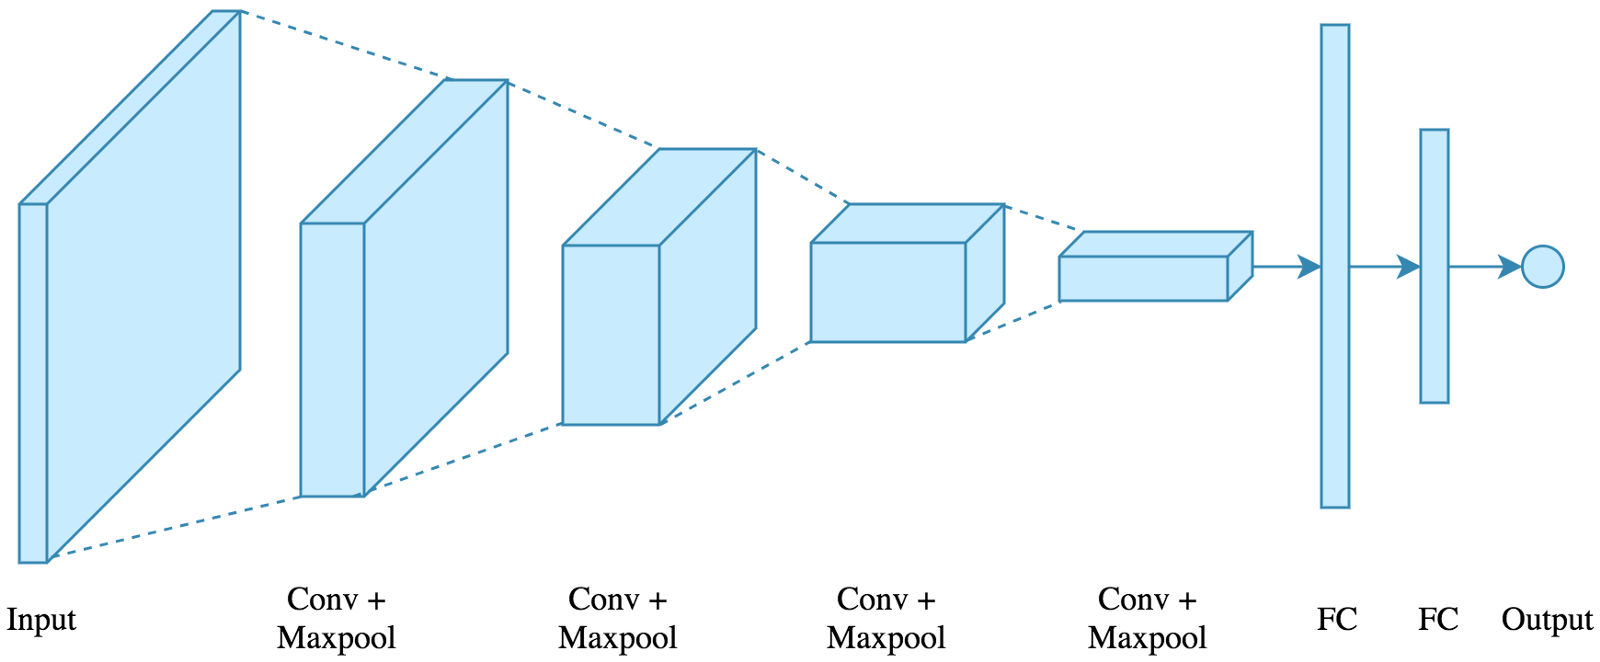
\includegraphics[scale=0.2,keepaspectratio=true,clip=true]{imagenes/MarcoTeorico/cnn_intuition.png}
  \caption{Arquitectura simplificada CNN.}
  % \\ (Adaptado de:https://towardsdatascience.com/understanding-input-and-output-shapes-in-convolution).} 
  \label{Fig:cnn_network}
\end{figure}




\subsubsection{Convolución}\label{sub:convolucion}
%https://www.superdatascience.com/blogs/convolutional-neural-networks-cnn-step-1-convolution-operation
Las principales operaciones de una \ac{cnn} están basadas en operaciones de convolución (ec. \eqref{eq:conv2}), la convolución son operaciones de producto y sumas entre las capas y los $n$ filtros (kernel) que generan  un mapa de característica como se mencionó anteriormente. La ventaja es que el mismo filtro permite extraer la misma característica en cualquier parte de la entrada, con esto se consigue reducir el número de conexiones y el número de parámetros a entrenar. En imágenes nos interesa usar la operación de convolución sobre más de un eje,  si tenemos una imagen $I$ y un kernel $K$ de dos dimensiones podemos definir como:

\begin{equation}\label{eq:conv2}
    G(i, j) = (I ∗ K)(i, j) = \sum_{m} \sum_{n} I(m, n) K(i - m, j - n).
\end{equation} 

$G$ será la matriz de salida denominada mapa de característica, para los valores de $i, j$ perteneciente a indices  de la matriz y $m, n$ corresponde a indices de filas y columnas de la imagen $I$.

% NOTA https://d2l.ai/chapter_convolutional-neural-networks/why-conv.html, 


En la figura (a) \ref{Fig:filter} tenemos de ejemplo una matriz de entrada y un filtro también denominado \textit{kernel}, en este caso un kernel (filtro) es de $3x3$ que se aplica a la matriz de entrada. La operación de convolución se realiza deslizando el kernel sobre la matriz de entrada del cual para cada ubicación realizamos una multiplicación de matrices y sumamos, el resultado de la suma sera nuestro nuevo \textit{mapa de característica} como se muestra (b) \ref{Fig:filter}.

\begin{figure}[htbp]
\centering
\subfigure[]{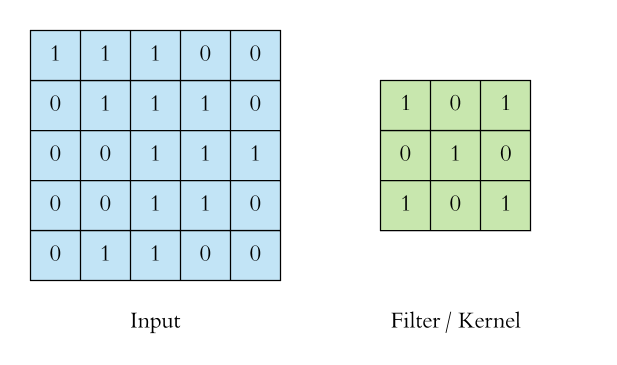
\includegraphics[scale=0.35]{imagenes/MarcoTeorico/convoluc_1.png}}%\\ (Adaptado de:https://www.superdatascience.com/blogs/)}
\subfigure[]{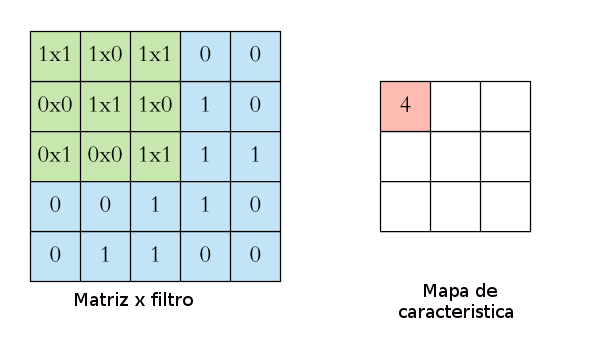
\includegraphics[scale=0.35]{imagenes/MarcoTeorico/convoluc_2.png}}%\\ (Adaptado de:https://www.superdatascience.com/blogs/)

\caption{(a) Matriz de entrada y filtro de convolución (b) Resultado de la operación de convolución.}\label{Fig:filter}
\end{figure}


Las \ac{cnn} desarrollan detectores de múltiples características y las utilizan para desarrollar varios mapas de características que se conocen como capas convolucionales, a través de estos mapas de característica la red determina qué  considera importantes para poder escanear imágenes y clasificarlas con mayor precisión.
%https://www.scribd.com/document/271869018/Convolucion-con-CNN
\subsubsection{Pooling}\label{sub:pooling}

%https://towardsdatascience.com/applied-deep-learning-part-4-convolutional-neural-networks-584bc134c1e2
Luego de las operaciones de convolución (sec:\ref{sub:convolucion}) usualmente utilizamos una capa llamada \textit{pooling}, esta capa se utiliza para reducir la dimensionalidad. La reducción de dimensionalidad nos permite reducir el número de parámetros que por consiguiente nos hará disminuir el tiempo de entrenamiento.

El tipo de técnica mas común utilizada es \textit{max pooling} que toma el valor máximo de la ventana permitiendo reducir el tamaño del \textit{mapa de característica} sin perder información, en la figura siguiente \ref{Fig:Pooling} se visualiza a modo de ejemplo el resultado de usar \textit{max pooling} de 2x2 con un \textit{stride} de 2.

\begin{figure}[H]
 \centering
  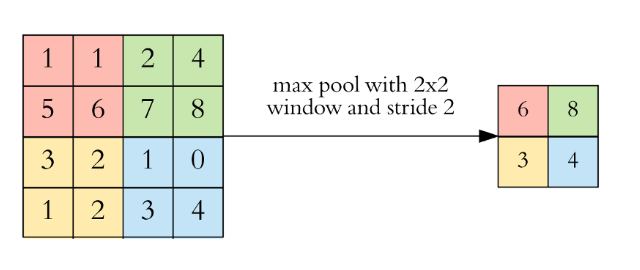
\includegraphics[scale=0.4,keepaspectratio=true,clip=true]{imagenes/MarcoTeorico/pooling_1.png}
  \caption{Pooling.} \label{Fig:Pooling}%\\(Adaptado de:https://towardsdatascience.com/applied-deep-learning)
\end{figure}

En las arquitecturas \ac{cnn} (sec:\ref{sub:arquitecturacnn}) normalmente la capa de pooling son ventanas de 2x2 con stride de $2$ mientras que las capas de  convolución se realizan con ventanas de $3x3$ y stride de $1$. 

\subsubsection{Función de activación}\label{sub:relu}
%https://towardsdatascience.com/activation-functions-neural-networks-1cbd9f8d91d6
%https://www.analyticsvidhya.com/blog/2017/10/fundamentals-deep-learning-activation-functions-when-to-use-them/
Las funciones de activación es una característica  importante de las \ac{cnn}, estas funciones básicamente deciden si una neurona debe ser activada o no, es decir si la información que la neurona está recibiendo es relevante para la operación dada o si se debe ignorar. Una vez que los \textit{mapas de característica} se extraen de la capa de convolución el siguiente paso es moverlos a una capa de activación. Existen diversos métodos que cumplen esta tarea, la mas utilizada en  \ac{cnn} son las capas de activación ReLU (Rectified Linear Unit), las  ReLU son operaciones punto a punto, las capas ReLU generalmente se acoplan con capas convolución. La función ReLU retorna 0 si existe un valor negativo de entrada mientras que retorna el mismo valor para cada valor positivo, en la figura  \ref{Fig:relu} vemos la forma que toma la función.

\begin{figure}[H]
 \centering
  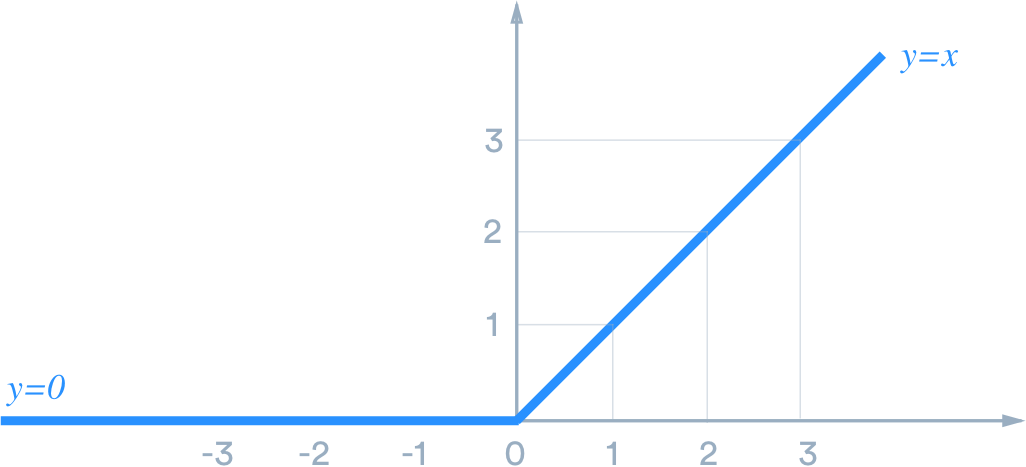
\includegraphics[scale=0.25,keepaspectratio=true,clip=true]{imagenes/MarcoTeorico/ReLU_1.png}
  \caption{ReLU (Rectified Linear Unit).}% \\ (Adaptado de: https://towardsdatascience.com/activation-functions-neural-networks)} 
  \label{Fig:relu}
\end{figure}

%Ejemplo aplicado de una ReLU a un \textit{mapa de característica} \ref{Fig:relu2}:
%\begin{figure}[H]
% \centering
%  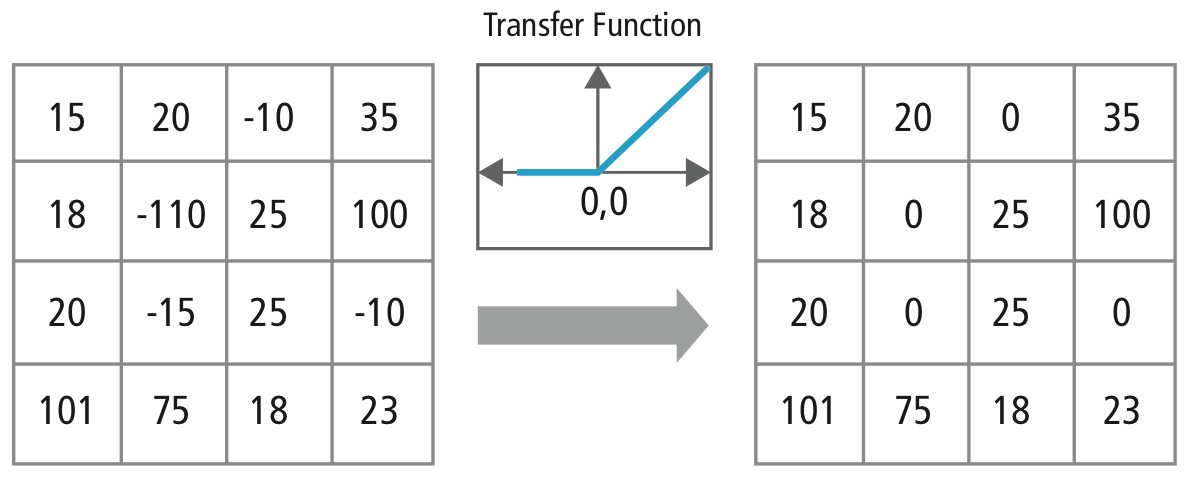
\includegraphics[scale=0.2,keepaspectratio=true,clip=true]{imagenes/MarcoTeorico/ReLU_2.jpeg}
%  \caption{Ejemplo ReLU  \\(Adaptado de: https://towardsdatascience.com/activation-functions-neural-networks)} \label{Fig:relu2}
%\end{figure}

La principal ventaja de usar la función ReLU sobre otras funciones de activación es que no activa todas las neuronas al mismo tiempo, si la entrada es negativa la convertirá a cero y la neurona no se activará esto significa que en un momento dado solo unas pocas neuronas se activan por lo que la hace eficiente y fácil de calcular.


\subsubsection{Capas totalmente conectadas}\label{sub:fully_connected}
%https://adeshpande3.github.io/A-Beginner%27s-Guide-To-Understanding-Convolutional-Neural-Networks/
% https://www.oreilly.com/library/view/tensorflow-for-deep/9781491980446/ch04.html

En las \ac{cnn} luego de las combinación de capas de convolución, ReLU y pooling agregamos capas llamadas totalmente conectadas, por su nombre en ingles \textit{fully conected}.
Las fully conected son las capas más básicas ya que todas las neuronas de entrada están conectadas a cada neurona de salida, una capa fully connected  es aquella en donde cada dimensión de salida  depende del valor de entrada a la red, esta red se basan en una combinación lineal (ec.\eqref{eq:fully-conected2}) de las variables de entrada que se transforma mediante una función de activación no lineal.


\begin{equation}\label{eq:fully-conected2}
a_j = \sum_{i=1}^D w_{ji}  x_i + w_{j0}.
\end{equation}
$ a_j$  se conoce como capa de activación para los pesos $w_{ji}$ y dado los valores de entrada ${x_1,...,x_d}$, en esta red hay  $ D$ entradas como $M$ unidades ocultas. La activación de la unidad  $ a_j$ se obtiene luego de la suma de la transformación lineal usando una función de activación $ g(.)$, ReLU por ejemplo, esto nos da que la salida de una \textit{fully conected} tendrá la forma de  \eqref{eq:output-fully-conected}.

\begin{equation}\label{eq:output-fully-conected}
z_j = g(a_j).
\end{equation}

Básicamente, una capa \textit{fully conected} observa características de alto nivel que se relacionan con una clase en particular y tiene pesos particulares para que cuando al calcular los productos entre los pesos y la capa anterior obtendrá las probabilidades correctas para las diferentes clases. Las capas fully conected desempeñan  la tarea de clasificación mientras que las capas convolucionales actúan como extractores de características.

%\begin{figure}[H] \centering
%  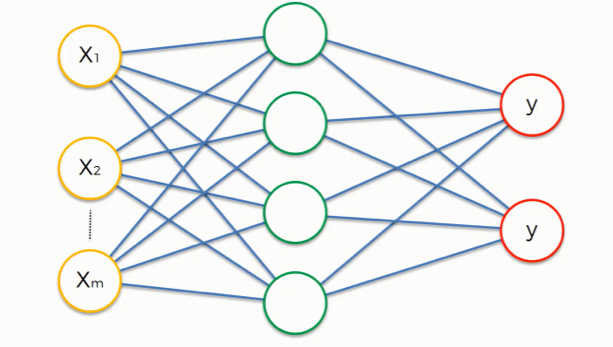
\includegraphics[scale=1,keepaspectratio=true,clip=true]{imagenes/MarcoTeorico/fully_conected.png}
%  \caption{Capas totalmente conectadas (Fully conected leyers) \\ (Adaptado de: https://adeshpande3.github.io)}\label{Fig:fully_conected}
%\end{figure}


%https://ahmedbesbes.com/understanding-deep-convolutional-neural-networks-with-a-practical-use-case-in-tensorflow-and-keras.html


\subsection{Arquitecturas de redes convolucionales}\label{sub:arquitecturacnn}
%https://towardsdatascience.com/neural-network-architectures-156e5bad51ba
%https://www.researchgate.net/publication/%309455781_Comparacion_de_Arquitecturas_de_Redes_Neuronales_Convolucionales_para_la_Clasificacion_de_Imagenes_de_Ojos
La arquitectura de una red neuronal es la forma en que se organizan  las neuronas en su interior, estas neuronas se agrupan formando capas que pueden llegar a tener diferentes características. Partiendo de los conceptos visto en la sección anterior (sec:\ref{sub:cnn})  vamos a entrar en detalle de diferentes modelos de arquitectura que existen actualmente.

\par \textbf{LeNet5} \citep{lenet} Fue una de las primeras \ac{cnn} que impulso el campo de \ac{dl}, la principal idea de esta red es que determinadas característica se distribuyen sobre toda la imagen, de esta manera convoluciones con los mismos parámetros pueden extraer de manera eficiente esas mismas características en toda la imagen en múltiples locación. LeNet5 esta formada por 3 capas usando la capa de convolución para extraer las características espaciales de la imagen, en general esta red fue el origen de muchas de las arquitecturas modernas.

\par \textbf{AlexNet} \citep{alexnet}: Esta arquitectura surgió en el 2012 ganadora de la competición \textit{ImageNet}\footnote{http://www.image-net.org/challenges/LSVRC/}. El problema resuelto en la competición era poder clasificar una imagen dentro de 1000 categorías. Cuenta con 60 millones de parámetros y 650.000 neuronas, AlexNet consta de 5 capas convolucionales con diferentes kernel que extraen diversas característica de la imagen  y 3 capas fully connected. Una importante característica es el uso de la función ReLU,  AlexNet demostró que al usar la no linealidad ReLU,  podrían entrenarse mucho más rápido que  funciones de activación como  tanh o sigmoide.

\begin{figure}[H]
 \centering
  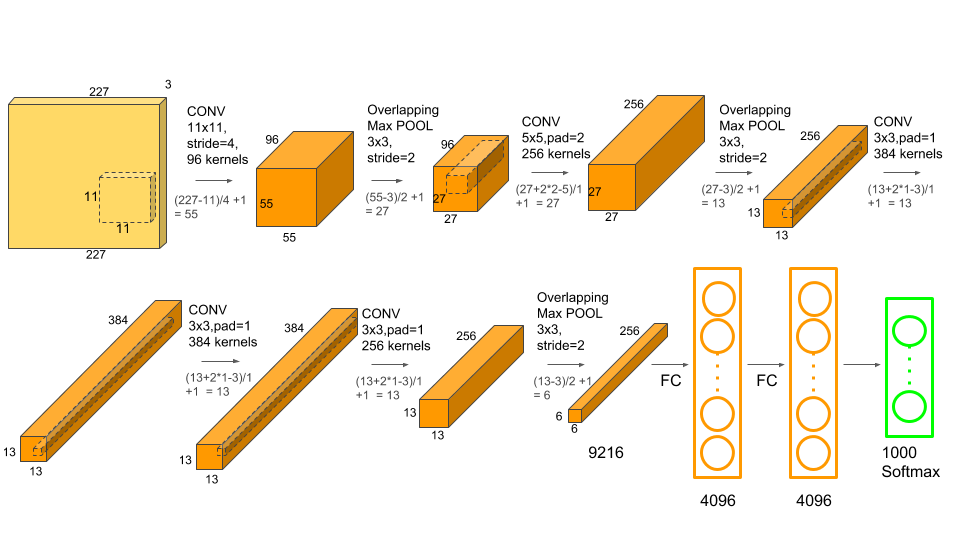
\includegraphics[scale=0.4,keepaspectratio=true,clip=true]{imagenes/MarcoTeorico/AlexNet-1.png}
  \caption{Arquitectura AlexNet \citep{alexnet}.}
	\label{Fig:alexnet}
\end{figure}


\par \textbf{VGG} \citep{vgg} Esta arquitectura se caracteriza por ser la primera en utilizar filtros 3 × 3 mucho más pequeños en cada capa convolucional y ademas los combinaron como una secuencia de convoluciones. La principal contribución de VGG, ganadora de la competición en 2014 de \textit{ImageNet}, es mostrar que la precisión de la clasificación y localización de un objeto en una imagen puede mejorarse al aumentar la profundidad de la \ac{cnn}.

\begin{figure}[H]
 \centering
  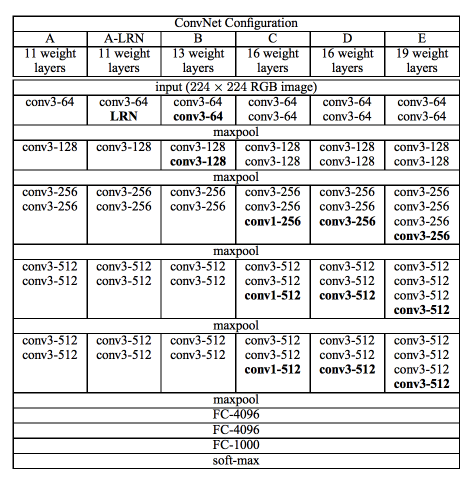
\includegraphics[scale=0.6,keepaspectratio=true,clip=true]{imagenes/MarcoTeorico/vgg.png}
  \caption{Arquitectura VGG \citep{vgg}.}
	\label{Fig:vgg}
\end{figure}

\par \textbf{GoogleNet} \citep{googlenet} El principal objetivo de esta arquitectura desarrollada es mejorar la utilización de recursos computacionales, esto lo logra definiendo módulos llamados, \textit{módulos inception}, y aumentando la profundidad y el ancho de la red. 
\begin{figure}[H]
 \centering
  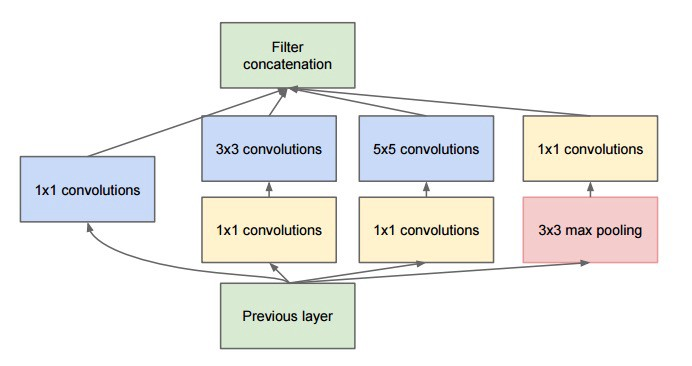
\includegraphics[scale=0.5,keepaspectratio=true,clip=true]{imagenes/MarcoTeorico/inception-1.jpg}
  \caption{Arquitectura GoogleNet: modulo Inception \citep{googlenet}.}
  	\label{Fig:inception}
\end{figure}
Como se puede ver en la imagen anterior \ref{Fig:inception} se diseño módulos para luego agruparlos uno arriba de otro, GoogleNet usa un nuevo termino llamado \textit{Bottleneck layer} que permite reducir el numero de características y sus operaciones 

\par \textbf{ResNet} \citep{resnet_a} Es otro tipo de arquitectura nombrada \textit{"Deep Residual Learning"}, a partir de mapeo subyacentes de $x y H (x)$, es posible aprender la diferencia entre los dos, que es el \textit{residuo} y, posteriormente ajustar el último a la entrada siendo el residuo $F(x) = H(x) - x$.

\begin{figure}[H]
 \centering
  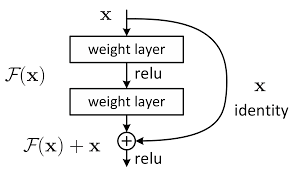
\includegraphics[scale=0.6,keepaspectratio=true,clip=true]{imagenes/MarcoTeorico/resnet.png}
  \caption{ResNet: \textit{Residual block \citep{resnet_a}.}}
	\label{Fig:inception}
\end{figure}


En el estado del arte actual existen diferentes variantes que parten de la idea principal de cada arquitectura mencionada anteriormente como: ResNet50, ResNet101, GoogleNet(InceptionV1, InceptionV3), entre otras. 

En la  figura \ref{Fig:cnn-analisis} se muestra un análisis realizado por \cite{Analysis_deep_network} en donde se compara la complejidad de las arquitecturas existentes en relación a su \textit{accuracy}, los círculos en el grafico representan la cantidad de parámetros de cada red, como se puede ver las redes \textit{VGG} son mucho mas costosas en relación a los costos computacionales como a la cantidad de parámetros que se debe entrenar. Por otro lado podemos ver con las demás arquitecturas tienden a mejorar su \textit{accuracy} a mayor costo computacional y numero de parámetros.
%https://www.deeplearningitalia.com/guia-para-arquitecturas-de-redes-profundas/

\begin{figure}[H]
 \centering
  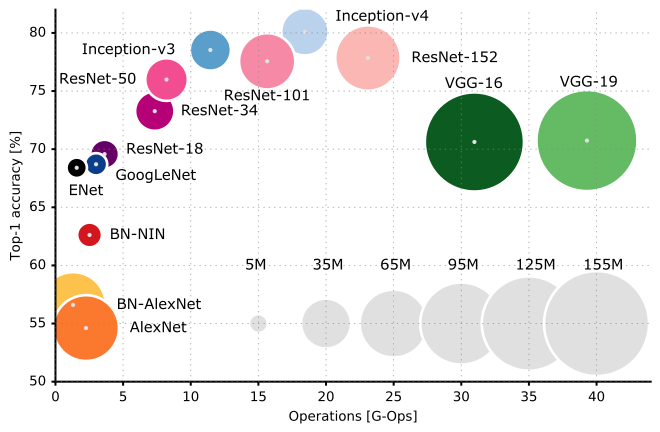
\includegraphics[scale=0.5,keepaspectratio=true,clip=true]{imagenes/MarcoTeorico/cnn-analisis.png}
  \caption{Análisis CNN, \citep{cazani_grap}.}\label{Fig:cnn-analisis}
\end{figure}



\subsection{El problema de la detección}\label{sub:problema_deteccion}


Las redes neuronales convolucionales como se desarrollo previamente nos permiten extraer información de una imagen, a partir de esta información extrída poder clasificarla. En un problema de detección ademas de clasificar la imagen necesitamos saber en que posición (coordenadas) de la imagen se encuentra el objeto de interés; los objetos en una imagen de una clase particular son altamente variables es decir se presenta el problema que el objeto puede variar en iluminación, cambios en la posición de la cámara y tamaño del objeto, para abordar este problema existen diversas técnicas una de ellas es por medio de un algoritmo de ventana deslizante, \textit{sliding windows} por su denominación en ingles. Sliding windows es un método para detectar objeto en una imagen, este método utiliza una ventana definida previamente que se basa en recorrer la imagen de izquierda a derecha y desde arriba a abajo dando pasos de $N$ píxeles definidos previamente. Este técnica puede ser considerada con diferentes tamaños de ventanas o con diferentes niveles de resolución convirtiendo la imagen en pirámide para la solución del problema de escala. 

El principal inconveniente de sliding windows es el costo computacional que conlleva ya que debe recorrer toda la imagen para encontrar el objeto de interés, generalmente los objetos no se presentan de un tamaño fijo en toda la imagen al aplicar esta técnica puede suceder que la ventana no coincida con el tamaño de ventana definido previamente, entonces se debe crear imágenes en pirámide para poder resolver el problema de escala como se menciona anteriormente; para dar un ejemplo en una imagen de $640 x 480$ píxeles con tamaño de ventada de $ 3 x 3$ y un salto de $2$ se deberían evaluar en el orden de $10^3$ ventanas en la imagen.

Existen diversos algoritmos mucho mas eficientes en termino de tiempo y reconocimiento de objeto que sliding windows estos son llamados regiones propuestas, \ac{rp} por su denominación en ingles, los métodos de regiones propuestas toman una imagen de entrada y retornan una región, bounding box,  que probablemente contengan algún objeto de interés en la imagen; los bounding box retornado por algunos de los métodos de regiones propuestas habrá al menos uno que contenga o se acerque al objeto de interés que estamos buscando dentro de la imagen.

% las regiones con alta probabilidad seran aquellas que contengan el objeto que estamos buscando, luego podemos clasificarla usando algun modelo como SVM.ZZZZ https://www.learnopencv.com/selective-search-for-object-detection-cpp-python/
Luego de generar las regiones propuestas extraemos las características de la imagen por medio de una \ac{cnn}, a partir de las salidas de esta extracción de característica, \textit{feature extraction} por su denominación en ingles, se utilizará algunos de los métodos de clasificación desarrollado en (sec:\ref{sub:clasificadores}) en la cual la salida serán los bounding box identificado con alguna probabilidad de que contenga o no el objeto que estamos buscando. Como siguiente paso debemos  asegurarnos que los bounding box no estén duplicados, es decir que no representen la misma información que otra región; para eliminar regiones duplicadas utilizamos el método de supresión de no máximos (NMS, pos sus siglas en ingles) (sec:\ref{sub:nonmaximumsuppression}) que a partir de un umbral previamente definido nos permite eliminar regiones duplicadas en la detección.


%Un pipeline básico de detección tiene la siguiente estructura \ref{fig:pipeline-deteccion}.
%\begin{figure}[H]\centering
%  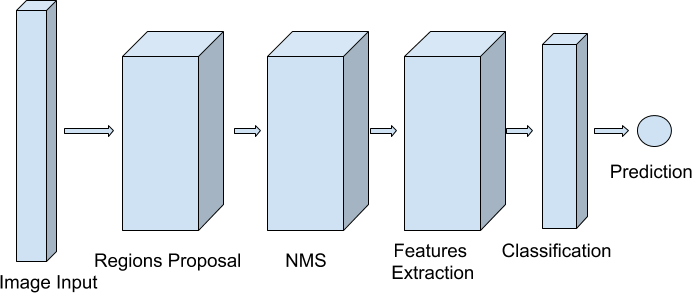
\includegraphics[height=5cm,keepaspectratio=true,clip=true]{imagenes/MarcoTeorico/pipeline-deteccion.png}
%  \caption{Pipeline de detección}\label{fig:pipeline-deteccion}
%\end{figure}

\subsubsection{Regions proposal} \label{sub:regions-proposal}

Regions proposal son un conjunto de métodos que permiten extraer regiones dentro de la imagen siguiendo algunas características similares como contorno, color, etc. El proceso metodológico básico es el siguiente: dada una imagen de entrada por medio de algún método se busca generar un conjunto de regiones candidatas que serán localizadas en un bounding box, el bounding box es la región de interés que probablemente contengan algunos objetos de interés para la detección (fig: \ref{Fig: propsalregion}); estos métodos permiten tener bounding box de diferentes escalas los que nos ayuda a poder localizar objetos de diferentes tamaños, los objetos de interés detectados serán los que posteriormente vamos a utilizar para realizar la clasificación; como podemos observar en la figura de ejemplo \ref{Fig: propsalregion} como se generan los bounding boxes en la imagen.

\begin{figure}[H] \centering
  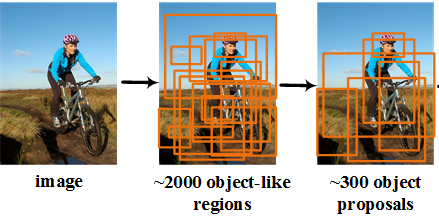
\includegraphics[scale=0.6,keepaspectratio=true,clip=true]{imagenes/MarcoTeorico/regionProposal.png}
  \caption{Regiones propuestas aplicado a una imagen con diferentes valores de regiones encontradas, \citep{regions_proposal_gr}.}
	\label{Fig: propsalregion}
\end{figure}

En el estado del arte existen diversas técnicas para obtener las regiones candidatas \citep{proposal}, en esta tesis  solo se realizaron pruebas con los  los métodos de: \textit{Edges Boxes} y \textit{Selective Search}. El método de Edges Boxes  \citep{edges} es un método para la generación de regiones candidatas a partir de los bordes detectados; utilizando estructuras de datos eficientes se pueden evaluar millones de boxes (cajas) candidatas en una fracción de segundo en donde los bordes proporcionan una representación simplificada pero informativa de una imagen. Los algoritmos para la detección de bordes tradicionales utilizan una variedad de métodos para calcular gradientes de color, en el caso de los nuevos enfoques además utilizan múltiples características como entrada incluyendo brillo, color, textura y  escalas de la imagen. Este método evalúa las cajas candidatas utilizando un enfoque de ventana deslizante, similar a la detección de objetos tradicionales \textit{sliding windows} en el cual para cada posición del objeto evaluamos, escala y relación generando una puntuación (score) que indica la probabilidad de que un objeto esté presente en el bounding box.

%\subsubsection*{Edges Boxes} \label{sub:edgesboxes}En la figura \ref{Fig: edges} podemos ver de manera simplificada los pasos del método;  en la parte inferior de la imagen \ref{Fig: edges} vemos que luego de varios operaciones identifica regiones que podrían ser de interés.

%\begin{figure}[H]
% \centering
%  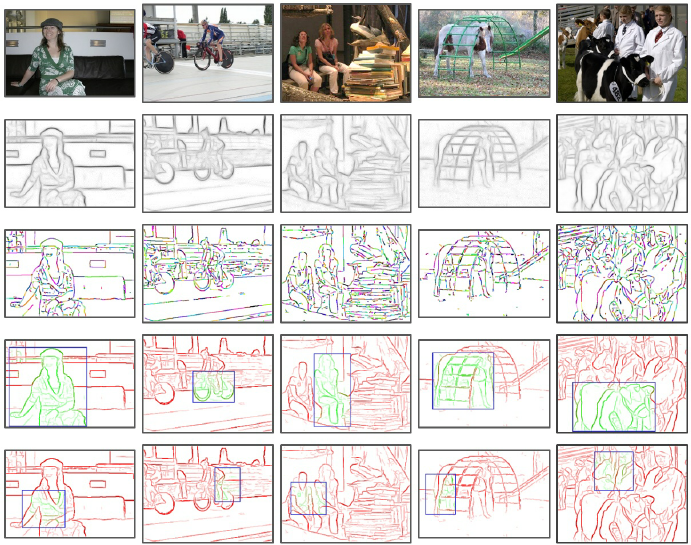
\includegraphics[scale=0.3,keepaspectratio=true,clip=true]{imagenes/MarcoTeorico/edges.png}
%  \caption{Ejemplo proceso detección de bordes \\ (Adaptado de:\citep{edges})}
%	\label{Fig: edges}
%\end{figure}

El método de \textit{Selective Search} \citep{selectivesearch} es un método de \ac{rp} que  permite obtener regiones candidatas realizando una búsqueda exhaustiva aplicando segmentación sobre la imagen. La segmentación  en procesamiento de imágenes consiste en dividirla en grupo de píxeles u objeto. El objetivo es simplificar la representación logrando que sea mas significativa, fácil de analizar y capturar todas las ubicaciones de objetos posibles; en lugar de una sola técnica para generar ubicaciones diversifica la  búsqueda y usa  una variedad de particiones de imágenes complementarias para tratar con tantas condiciones de imagen como sea posible.
Las estrategias usadas en este método es \textit{capturar todas las escalas}: los objetos pueden estar en cualquier escala de la imagen, es por esto que se toma en cuenta todas las escalas, \textit{diversificación}: No existe una sola estrategia sino que una región puede formar un objeto solo por color o textura y \textit{computo rápido}: Esta es una de las estrategias principales debido a que el objetivo es producir un conjunto de regiones propuesta de manera eficiente y sin un costo computacional alto.

\begin{figure}[H]
 \centering
  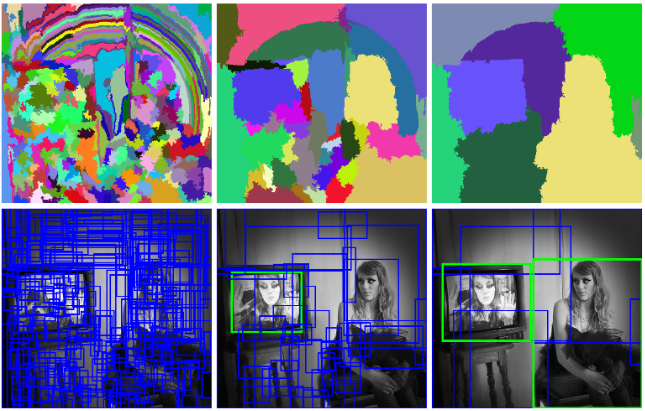
\includegraphics[scale=0.4,keepaspectratio=true,clip=true]{imagenes/MarcoTeorico/selectivesearch.png}
  \caption{Segmentación por el método de \textit{Selective Search} con diferentes valores de umbrales \\ \citep{selectivesearch}.}
	\label{Fig: overlapping}
\end{figure}

Luego de las extracciones de regiones candidatas obtenidas por algunos de los métodos nombrados anteriormente, debemos obtener las características significativas que representan cada región dada. Una  característica es algo que se diferencia del resto en un conjunto de datos, esa diferencia nos permite agruparlas de acuerdo a alguna similitud entre las mismas. El objetivo principal de la  extracción de características, \textit{feature extraction} por su denominación en ingles, es representar los datos como un conjunto reducido de característica que describen de manera eficiente sus principales atributos. Para poder realizar esta tarea utilizamos  las redes neuronales convolucionales (sec:\ref{sub:cnn}) que  permiten extraer información de la imagen para luego utilizar estos atributos obtenidos y agruparlos según algún criterio previamente establecido. 



%\subsubsection*{Selective Search} \label{sub:selectivesearch}

%\subsection{Extracción de características}\label{sub:features-extraction}

%Luego de las extracciones de regiones candidatas obtenidas por algunos de los métodos nombrados en la sección anterior (Sec:\ref{sub:regions-proposal}), debemos extraer las características significativas que representan cada región dada. Una  característica es algo que se diferencia del resto en un conjunto de datos, esa diferencia nos permite agruparlas de acuerdo a alguna similitud entre las mismas. El objetivo principal de la  extracción de características, \textit{feature extraction} por su denominación en ingles, es representar los datos como un conjunto reducido de característica que describen de manera eficiente sus principales atributos. Para poder realizar esta tarea utilizamos  las redes neuronales convolucionales (Sec:\ref{sub:cnn}) que  permiten extraer información de la imagen para luego utilizar estos atributos obtenidos y agruparlos según algún criterio establecido. 


\subsection{Non-maxima suppression}\label{sub:nonmaximumsuppression}

El método de supresión de no máximos (NMS) es un post-procesamiento frecuente en el contexto de la detección de patrones. El algoritmo  \ac{nms} se encarga de eliminar regiones que estén superpuestas entre si como se muestra en la figura  \ref{Fig: overlapping}.

\begin{figure}[H]
 \centering
  \includegraphics[scale=0.6,keepaspectratio=true,clip=true]{imagenes/MarcoTeorico/regions_prop.png}
  \caption{Superposición entre las regiones A y B.} \label{Fig: overlapping}
\end{figure}

Para poder eliminar detecciones redundantes calculamos un valor denominado  \textit{IoU}, intersección sobre unión,  este valor nos indica el solapamiento, \textit{overlapping} ,  entre diferentes regiones cercanas como se muestra en la figura \ref{Fig: interseccion}. El algoritmo de \ac{nms} puede ser formulado como una búsqueda de los máximo locales en donde el máximo local es  mayor que todos sus vecinos; el algoritmo selecciona aquellas detecciones con un \textit{puntaje} (IoU) alto y elimina los vecinos mas cercanos ya que es muy probable que cubran el mismo objeto \citep{nms2}.

\begin{figure}[H]
 \centering
  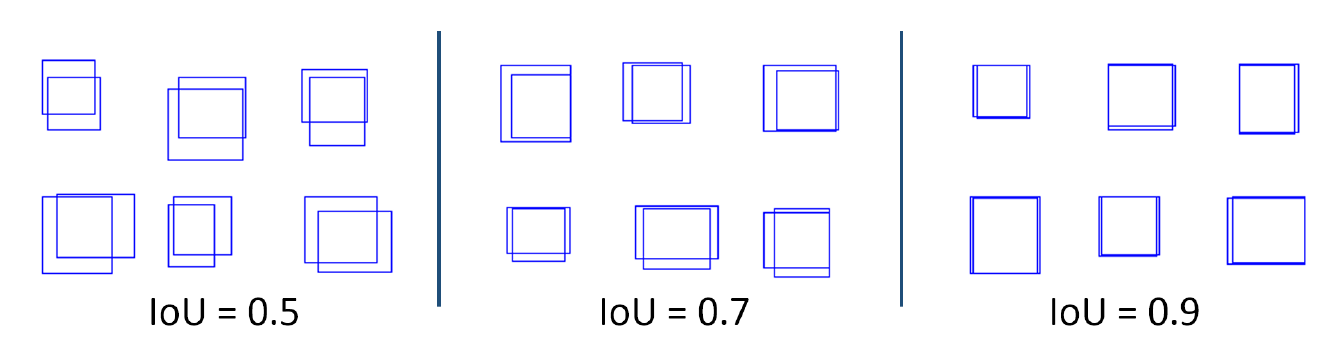
\includegraphics[scale=0.3,keepaspectratio=true,clip=true]{imagenes/MarcoTeorico/overlapping.png}
  \caption{IoU con diferentes valores de puntajes \citep{bishop}.}\label{Fig: interseccion}
\end{figure}

Dependiendo del valor de IoU  obtenido podemos usar un umbral para  eliminar las detecciones redundantes y lograr una mayor optimización  en el reconocimiento; para obtener una visión mas general del método podemos ver la siguiente figura \ref{Fig: nonmaximumsuppression}. 

En un pipeline de detección las técnicas de \ac{nms}  se utilizan para eliminar detecciones redundantes luego de la clasificación esto nos permite reducir el numero de detecciones a solo una por cada región detectada.

\begin{figure}[H]
 \centering
  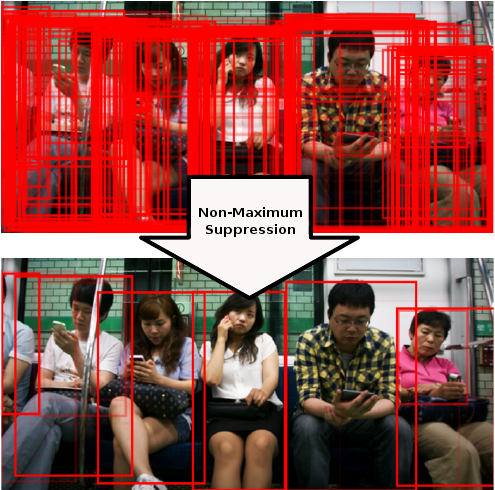
\includegraphics[scale=0.4,keepaspectratio=true,clip=true]{imagenes/MarcoTeorico/nms.png}
  \caption{\ac{nms} aplicado a una imagen, \citep{nms2}.}\label{Fig: nonmaximumsuppression}
\end{figure}

El siguiente algoritmo  \eqref{alg:nms} se visualiza el proceso llevado a cabo por \ac{nms} en la eliminación de regiones redundantes.  El algoritmo  recibe como entrada un conjunto de datos $\beta$ que indican la cantidad de regiones, $S$  indican el valor IoU de cada una de las regiones, por ultimo recibe un valor $N$ que  referencia el umbral utilizado para la  eliminación de las detecciones redundantes. 
%https://www.vision.ee.ethz.ch/publications/papers/proceedings/eth_biwi_01126.pdf
%D es un acumulador de bboxes
\begin{algorithm}[H]\caption{Non-Maxima Suppression}\label{alg:nms}

\begin{algorithmic}[1]
\State $\textbf{INPUT} : \beta = {b_1,..,b_n}, S = {s_1,..,s_n}, N_t$
%\State $\beta lista de bounding box.$
%\State $S puntaje obtenido por bounding box.$
%\State $N_t umbral definido de Non-maxima supression.$
\State $ \textbf{BEGIN} $
\State $D \gets \{\}$
\While {$\beta \neq empty$}
    \State $ m\gets  \argmax S $
    \State $ M \gets b_m $
    \State $ D \gets D \cup M; B \gets B - M $
    \For {$b_i$ to $\beta$}
        \If {$IoU(M, b_i) \geq N_t$}
            \State $ B \gets B - b_i; S \gets S - s_i $
\EndIf
\EndFor
\EndWhile
\State $\textbf{return}   D, S $
\State $\textbf{END}$
\end{algorithmic}
\end{algorithm}
